\chapter{Tools for the job}
\label{ch:tools}
\vspace{-1.3cm}

The previous chapters highlighted the need for a new software architecture that may constitute the foundational layer of distributed autonomous systems, and provided a solid set of requirements that can drive its design. Existing frameworks have been reviewed, some of which provided valuable insights and ideas about how to address some of the design challenges, but none ultimately offering the complete set of features required. Before presenting the design of the solution that this work proposes, it is important to delve further into a point that the previous discussion shed light onto: there are solutions available in the literature, in the industry, and in the open-source software community, that can be employed to address some of the key issues that the requirements identify. Following the computer science principle recalled in \Cref{sec:prb_requirements}, that is, to not reinvent the wheel, it is wise to review these tools and see how they can be integrated in the proposed solution. This chapter provides such an overview: for each tool, its motivations are shown by illustrating a problem that is common in the development of distributed autonomous systems, and then the tool itself is presented, along with a brief discussion of its features and limitations. Note that the aim of this work is to provide a general-purpose software architecture, so not all of the solutions presented in this chapter, as well as all the features that the proposed architecture has, may be necessary or even beneficial in every practical context. However, the goal is to provide a solution that can be adapted to a wide range of applications, as a good toolbox to have at hand, offering a set of features that can be configured and used as needed. Indeed, recalling that one of the requirements is also to develop an architecture that can be maintained over time, the intention is that the tools presented in this chapter are included because they represent valid solutions to the problems they address, which are relevant in this context, but since not a thing of this is set in stone each aspect of the proposed architecture can be subject to change in the future should the need arise.

\section{Inter-process communication: the middleware}
\label{sec:middleware}
When developing distributed systems composed of many modules, especially software ones, the transmission of data among them becomes a topic of paramount importance. Note that this issue concerns both transmissions happening between software modules running on the same host and on different hosts. Moreover, alongside this topic there is that of \emph{intra-process communication}, that is, the organization and regulation of data exchanges among different threads running in a same process. Examples of situations in which many software modules may coexist inside a single process, and why such a situation may be desirable, are presented and discussed in the following, for now let us focus on the general problem of inter-process communication and simply note that in the majority of the situations, this other problem can be solved by employing either the same tools that are used for inter-process communication, or simpler ones based on shared memory areas guarded by synchronization primitives.
One has, in general, to figure out a variety of issues such as the following:
\begin{itemize}
  \item \textbf{Data formatting}, \emph{i.e.}, how information that should travel from one module to another should be encoded and structured in packets or similar entities.
  \item \textbf{Data serialization and deserialization}, \emph{i.e.}, how packets should be transformed into a format that can be transmitted over a medium, which is usually some kind of point-to-point connection or a network.
  \item \textbf{Data transmission}, \emph{i.e.}, how packets should be sent and received, and how the system should react to errors or delays in the transmission; this also includes things like reliability requirements, that is, whether the system should guarantee that a packet is delivered, and how many times it should try to deliver it if it fails.
\end{itemize}
The points listed above are usually dealt with by employing a specific \emph{protocol}, that is, a predefined set of rules that regulate all those aspects of the communication. All the software that composes the system should adopt such protocol, which is usually implemented in a set of libraries that can be used in the code. However, dealing directly with networking protocols might slow down the development process: the host system configuration usually becomes very important, since all the operating systems involved must agree on the protocol implementation to support and use, and a lot of work may become necessary to proficiently use all the protocol APIs to achieve all the desired communication features and behaviors. Let us remember that this is not the original task: the goal is to develop a distributed autonomous system, and to write software for it, thus it would be desirable to have a tool that abstracts all the networking details and provides a simple and easy-to-use API that makes data transmission in software modules a straightforward operation, from both the coding and implementation points of view. This is where a particular kind of software, historically denoted by the term \emph{middleware}, comes into play. To grasp its importance in the context of this work, a step back in time is necessary.

In 1968, a conference sponsored by the Science Committee of the North Atlantic Treaty Organization (NATO) was held in Garmisch, Germany, on the topic of software development. Although not widely discussed, it was a historically significant event in this field: it provided a comprehensive overview of the design practices and methodologies used by leading companies in the growing and highly competitive field of computing. The goal was to identify standard strategies for addressing common problems. It should be noted that at that time, and for at least another fifteen years, there were virtually no standards in computer production and programming. Each company offered its own product developed from scratch, in both hardware and software. Standardization and collaboration among various manufacturers began only when information started being exchanged between different computers, first through storage media and later over the Internet, alongside a growing demand for new types of devices and standard formats to adopt when sharing data. A fairly complete transcription of the conference can be found in \cite{naur_software_1969}. It includes the first official mentions of several concepts well known today, such as \emph{component design} and \emph{unit testing}. However, of particular relevance to this work is the representation of the hierarchical structure of software presented by one of the speakers. This structure, valid even today with certain extensions, is illustrated in the inverted pyramid scheme shown in \Cref{fig:swpyramid}.
\begin{figure}[t!]
  \centering
  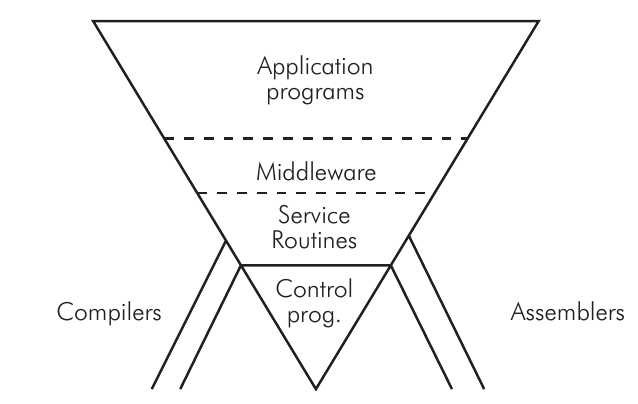
\includegraphics[width=.8\textwidth]{images/ch3/software_pyramid.png}
  \caption{Software organization in a general-purpose computer, as presented at the 1968 NATO conference on software engineering \cite{naur_software_1969}.}
  \label{fig:swpyramid}
\end{figure}
The idea is that a complex system is like an inverted pyramid: it cannot remain operational without adequate support provided by secondary components. These might be completely invisible to the end user and thus may be considered somewhat external, yet are of vital importance for the correct functioning of the whole: \emph{compilers} and \emph{assemblers}, for instance, which are programs that translate code written in a given language first into the target architecture's assembly language and then into binary machine language, typically generating an executable file at the end of the processing pipeline. These tools must be reliable and efficient, as the implementation of everything else depends on them. Next, we have the layers of \emph{Control Programs} and \emph{Service Routines}: these are what we today call the \emph{operating system} and \emph{device drivers}. They are typically developed with a strong dependence on the machine at hand, considering its specific characteristics, and heavily depend on the employed compilation tools. Their role is to provide an abstraction of the hardware that makes its use simple both for the end user, who interacts with applications, and for application developers themselves. The application software is precisely what we find in the topmost layer: programs that use the hardware more or less directly to provide various services to users. There is, however, an intermediate layer that is often overlooked because it was not always present or was difficult to characterize in the past: the \emph{middleware}. Situated between system software and application software, middleware found its first definition and characterization at the aforementioned conference. Initially conceived merely as a connective layer between current and \emph{legacy} software, middleware provides services and functionalities common to applications beyond what the operating system offers, building itself on top of it and abstracting its own implementation and protocol details. From the perspective offered by the topmost level of the inverted pyramid it appears as normal application software, often consisting of shared or dynamic libraries. Middleware typically offers services to programmers aimed at, \emph{e.g.}, data management, communication, and authentication. Therefore, middleware aids developers in building applications more efficiently by acting as a connective tissue between applications, data, and users. In distributed environments, middleware can facilitate the development and execution of large-scale applications. A typical service offered by middleware is a method for data exchange between applications, even across different devices, according to a common format referred to as an \emph{interface}, which is defined as needed. In general, the services offered by middleware are specified only in terms of their dynamics but can be implemented on different architectures and devices, functioning consistently while keeping their implementation hidden from both the application programmer and the end user. For example, when middleware handles communication between applications, it might position itself within the network stack between the transport and application layers\footnote{Considering the TCP/IP model, which is a four-layers reduction of the original seven-layers Open Systems Interconnection (OSI) model of the networking protocol stack.}. Today, middleware can be categorized into two types: that which operates in \emph{human time}, designed for direct use by human users (\emph{e.g.}, web services), and that which operates in \emph{machine time}, composed mainly of APIs that application developers can use to facilitate their work, benefiting from increased portability across a wide variety of devices. In light of all this, and considering the common difficulties faced when designing the software for a distributed autonomous system, it becomes clear how adopting communication middleware to solve the problem of data exchange among modules can simplify things: many functionalities that would have to be implemented from scratch would instead be offered by the middleware itself as services to be employed in the programs being developed. The selection of this particular class of middleware is again motivated by both the current trends in the software industry pertaining to the development of autonomous systems, and to the direct experience of the author in the field during this work.

The rest of this section will introduce three specific middlewares that are widely employed in the industry and in the open-source community, and that have become of pivotal importance in the two practical scenarios considered later in this work as a specialization of the proposed architecture: that of autonomous robotics and that of power plants. The first middleware is the \emph{Data Distribution Service} (DDS), which has been the first to provide a standard for data exchange in distributed systems, followed by the Zenoh middleware which addresses some of the limitations of DDS, and finally the \emph{Robot Operating System} (ROS), which is a middleware specifically designed for robotics applications. All these three components will be included in the architecture proposed in the following chapters, making some of its foundational layers.

\subsection{Data Distribution Service}
\label{sec:dds}
In 1989, eleven companies including Hewlett-Packard, IBM, Sun Microsystems, Apple Computer, and American Airlines, founded the \emph{Object Management Group} (OMG), a consortium that is still active in the field of computing with the goal of defining standards for industrial software. This effort aims to foster the integration of solutions from different vendors into unified ecosystems, covering a variety of applications and technologies. The purpose of the OMG is to establish, for every new type of software under consideration, a common model to be followed during its implementation, thus enabling and promoting its development and use on any potentially relevant platform. The group provides the industry with specifications only, not implementations. However, any team submitting a new specification must provide a potential implementation before it is accepted, intuitively to avoid defining impractical or useless standards. OMG member companies encourage the development of solutions that can interoperate immediately without any limitations.

One of the standards defined by the OMG is the \emph{Data Distribution Service} (DDS) \cite{pardo-castellote_omg_2003,schlesselman_omg_2004}. It specifies a particular type of middleware responsible for managing direct communications between computer systems, including the details of how data should be serialized, deserialized, transmitted, and routed, as well as how APIs should be structured for programmers to invoke these operations. Its definition has been carried over with the goal of allowing implementations to satisfy real-time determinism guarantees whenever necessary. Moreover, the goal of the DDS is to enable technologies, platforms, and devices from different vendors, operating in distinct contexts and locations, to immediately communicate, exchanging data for which only the format and minimal other attributes must be known beforehand. This facilitates the management of critical aspects, like performance and scalability of the various components and the network connecting them. Effectively, the DDS greatly simplifies what would otherwise be for the programmer a complex task of configuring networks and organizing data transmissions, which, as discussed, is one of the classic challenges faced during the development of a distributed autonomous system. As such, the DDS has become widely employed in industrial contexts ranging from manufacturing \cite{essers_evaluating_2014} to power grids \cite{saxena_distributed_2021}.

The middleware model follows a \emph{publish-subscribe} paradigm: entities involved in the communication declare their intent to transmit or receive packets of information, which are encoded according to appropriate interfaces, and are called informally \emph{publishers} or \emph{subscribers} and instantiated as \texttt{DataWriters} or \texttt{DataReaders} respectively. The publish-subscribe denomination arises from the way different transmissions are organized, from the programmer's perspective, into channels denoted as \emph{topics}. Topics are defined by:
\begin{itemize}
  \item a \textbf{name} that identifies the topic, generally encoded as a text string to be easy for programmers to remember and use;
  \item an \textbf{interface}, described using a specific language (\emph{e.g.}, an Interface Description Language (IDL)\footnote{The acronym IDL identifies a class of languages that allow the description of operational elements intelligible by different languages. Various IDLs exist, and in this context, DDS employs one to make the specification of a data packet format simple for programmers, although no specific IDL is mandated by the OMG standard.}), which specifies the content of a single data packet and how it is encoded.
\end{itemize}
Interfaces are intended as structured data types, \emph{i.e.}, data structures containing ordered fields of different types, ranging from simple integers and floating-point numbers to more complex structures like arrays and strings, or other interface types as well. One key aspect to consider is that, given an interface specification, the middleware will take care of generating the code necessary to serialize and deserialize data packets according to that interface, as well as to transmit and receive them over the network. This is a significant advantage, as it allows the programmer to focus on the data itself and on the logic of the application, without having to worry about the details of the network communication. Another key aspect to consider, which also makes the DDS very versatile, is that communications are asynchronous by nature: \texttt{DataWriters} publish data on a topic regardless of the presence of any \texttt{DataReader} listening on that topic. \texttt{DataReaders}, on the other hand, can subscribe at any time to a given topic and start receiving messages from that point on. The OMG DDS standard provides APIs for both synchronously waiting for new messages, as well as asynchronous notification and handling via \emph{callback}\footnote{A callback, in a software program, is a routine that gets called asynchronously, \emph{i.e.}, when an event occurs for which that callback is registered, and either an event handler or a job scheduler invoke such callback to process the event.} functions.

The behavior of any entity in a DDS network, and thus that of every transmission, can be configured by specifying a Quality of Service (QoS) policy for it \cite{corsaro_quality_2006}. A DDS QoS policy typically consists of items such as:
\begin{itemize}
  \item the \textbf{history policy}, which indicates whether all packets transmitted on a specific topic should be delivered or buffers, limited to a certain size, should be put in place and rotated in case of network congestion;
  \item the \textbf{history depth}, which is the depth of the finite queues optionally set in the previous point;
  \item the \textbf{reliability policy}, indicating whether communications should be managed by the middleware to ensure that all subscribers of a topic receive all packets transmitted by publishers, or packet drop and loss are allowed, thus enabling \emph{retransmissions} if necessary;
  \item the \textbf{durability policy}, allowing transmitted packets to be retained by publishers and delivered to subscribers that may connect later;
  \item the \textbf{deadline}, \textbf{lifespan}, \textbf{liveliness}, and \textbf{lease duration}, which are characteristic maximum times to determine when a packet has become outdated or an entity can be considered inactive.
\end{itemize}
Of course, there are default settings that are kept as consistent as possible across different implementations to ensure maximum compatibility. A complete scheme of a DDS network of applications can be found in \Cref{fig:ddsnet}.
\begin{figure}[t!]
  \centering
  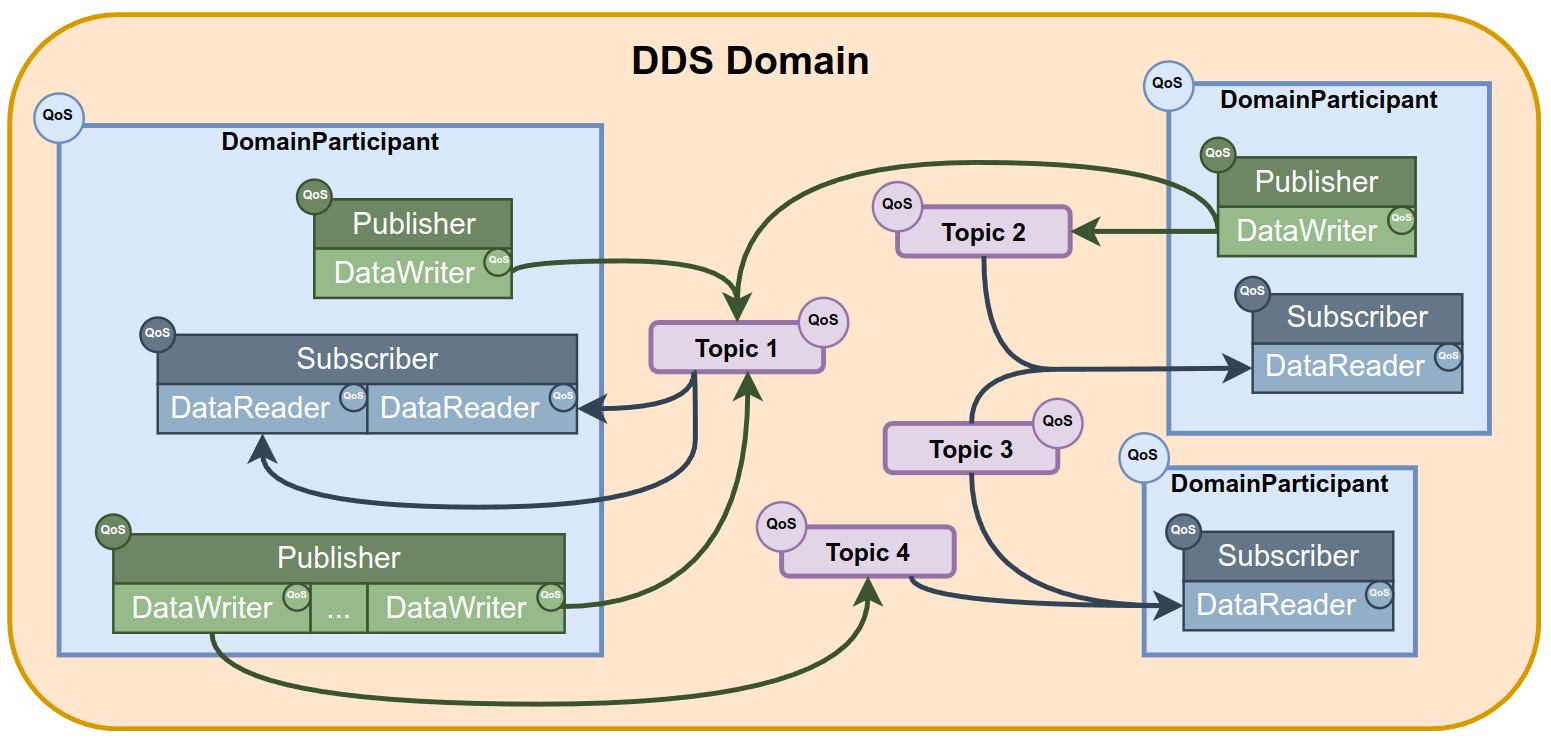
\includegraphics[width=.8\textwidth]{images/ch3/dds_domain.png}
  \caption{A network of applications using the DDS, each denoted by its own \texttt{DomainParticipant} \cite{eprosima_11_nodate}.}
  \label{fig:ddsnet}
\end{figure}

Even at this level, the significant simplification introduced by the DDS middleware becomes evident: with a relatively simple and quick configuration, issues such as choosing a transport protocol (\emph{e.g.}, Transmission Control Protocol (TCP) or User Datagram Protocol (UDP)) and developing software modules to use it for transmitting information encoded according to specific rules and formats can be immediately resolved. The DDS takes care of all tasks necessary to organize communications: from the most basic, such as message transmission, to more organizational tasks like publisher advertising and node discovery within the network, as well as flow control and retransmissions. It also handles publisher redundancy and other pathological situations—all in a way that is completely transparent to the programmer. DDS, in effect, makes it very simple to build distributed applications or networks of applications, as it hides and simplifies many management tasks, allowing the developer to be abstracted from factors that could otherwise prove complex to manage. Commercially available DDS implementations today offer API libraries in various languages, such as Ada, C, C++, C\#, Java, Python, Scala, Lua, Pharo, and Ruby, and since they are all built on the same standard, they are fully compatible and interoperable. There are also specifications concerning lower-level types of DDS, designed to be included in resource-constrained systems, such as embedded systems, while still maintaining compatibility with more comprehensive high-level implementations.

Communication modes, serialization, and deserialization of data are defined in the OMG standard called \emph{Wire Protocol}. Despite the broad scope of this specification, it is instrumental to highlight two key parts for the benefit of the following discussions.

\subsubsection{Discovery Module}
\label{sec:dds_discovery}
This module of the DDS includes protocols that allow different DDS instances running on network-connected systems to discover each other and organize potential communications from that point on. Generally, there are two such protocols:
\begin{itemize}
  \item \textbf{Participant Discovery Protocol (PDP)}, which allows DDS instances—each associated with a particular application running on a specific machine, hence called \emph{participants}—to announce their presence to others while simultaneously obtaining information about any other reachable participants.
  \item \textbf{Endpoint Discovery Protocol (EDP)}, which comes into play immediately after PDP, and relates to transmitting information about the \emph{endpoints} owned by the various participants. These endpoints, as publishers or subscribers, are deemed compatible if they share the same topic and interface, and if the QoS policies \emph{offered} by publisher entities satisfy the \emph{requests} of subscriber entities.
\end{itemize}
Implementations can choose to include, beyond the PDP and EDP protocols defined by the standard\footnote{These are known as \textbf{SPDP} and \textbf{SEDP}, respectively, where ``S'' stands for ``Simple''.}, proprietary versions. If two instances initiating communication have at least one PDP and one EDP in common, they can exchange information and complete the discovery process.

These protocols would be located at the Internet Protocol (IP) level in a network stack, and can be implemented in either \emph{unicast} or \emph{multicast}, depending on whether all participants are known in advance or not. In the former case, preliminary network configuration is required to preset the addresses and port ranges of all involved machines, while in the latter, the protocols will automatically manage everything as soon as the DDS instances are launched. The potentially vast operational scale of these solutions has made DDSs attractive for mission-critical areas such as military and logistics, although, for now, relying entirely on the Internet for such communications is not advisable. Unless predefined configurations are in place, it is necessary for every network device along the path between two participants to support multicast and not block such transmissions.

\subsubsection{Platform Specific Model}
\label{sec:dds_psm}
This model establishes how data of different formats and encodings should be serialized, transmitted, and deserialized in a uniform manner across all possible implementations and platforms. In an IP network, all data packets are transported over UDP. Whether the endpoints are associated using multicast or unicast, the Discovery Module's protocol opens UDP \emph{sockets} for them with well-defined port numbers, which depend on:
\begin{itemize}
  \item the \textbf{domain ID}, a numerical constant that selects a range of UDP ports in the implementation, allowing applications using DDS to communicate simply by specifying the same domains; multiple domains can coexist even on a single machine;
  \item the \textbf{base range} of UDP ports available in the system;
  \item the \textbf{participant ID}, a unique identifier for an instance within a machine;
  \item any other \textbf{manual}, specific configurations.
\end{itemize}
One may wonder why UDP is used for data transport. The reasons are similar to those in other contexts where a deterministic behavior is desirable: UDP is a basic, best-effort protocol without any communication management features beyond simple transport between endpoints. As such, it is lightweight and supported by a wide variety of devices and platforms. This simplicity gives UDP implementations complete predictability, excluding the unpredictability of the network itself, and natural scalability. Therefore, it is the best choice for real-time systems as well as for the development of this type of software.

\subsection{Zenoh}
\label{sec:zenoh}
The Data Distribution Service middleware effectively solves the inter-process communication problem in distributed contexts, allowing applications to easily set up communication channels over a network of potentially very large scale. As the previous section clarified, it is particularly user-friendly from the point of view of the application programmer also because of its automatic configuration capabilities: thanks to the Discovery Protocol, DDS participants and their related entities can automatically discover each other and connect, without any prior network configuration required. If all of this seems too good to be true, that is because it actually is. Coming back to the origins of the DDS specification, one can see how they date fairly back in time: the first drafts of the protocols were redacted in the late 90s, while the first officially published implementations are from the early 2000s. In the meantime, the world of computing has changed a lot, and situations that were only theorized before are currently the norm. A wide variety of new technologies, which are all somehow related to networking, have seen the light of day in the meantime. As an example, consider the advent and diffusion of various high-bandwidth wireless networks like WiFi or 5G, which then led to other advancements like cloud computing, Internet of Things (IoT) and edge computing. All these technologies are nowadays part of the daily life of many people, and they have all contributed to shape the current scenario in information technology: digital devices are everywhere, on every scale, all interconnected at the same time using a variety of technologies and protocols. That is also what made distributed autonomous systems possible, but also changed the world into something much different than the one in which the DDS was born. When the OMG DDS standard was designed, networks were still made of cables and routers, with point-to-point links which finally allowed little to no packet loss, and connected devices which were different declinations of the same concept: a big computer. Nowadays, the term ``computer'' has a much broader meaning, and networks connect devices that operate on many different scales using multiple types of physical links. One of the few things that is common among all is that they all need to share large, if not huge, amounts of data among themselves. This is where the DDS starts to show its limitations: it was designed for a world where the network was a mostly reliable and predictable medium, and connected devices could be assumed to have a certain level of computational power and memory. This is not the case anymore, and the DDS is starting to show its age. The main limitations of the DDS are related to these exact contexts, and came up in the last five years due to its wide adoption in new contexts like that of autonomous robotics, where having multiple heterogeneous devices connected over a wireless, lossy\footnote{In this context, the adjective ``lossy'' denotes a packet switching network subject to \emph{packet loss}, \emph{i.e.}, the possibility that packets flying get dropped by the devices handling them because of network congestion or similar phenomena, in an attempt to preserve overall network functionality.} network is the norm. The most limiting factor of the DDS is, in fact, its intrinsic reliance on a network layer which requires little to no retransmissions. If this assumption is not met, communications based on the DDS can become very slow or even fail completely due to network congestion. This is mainly due to the fact that the Discovery Protocol has not been designed with this situation in mind, so that it requires a number of multicast transmissions that grows exponentially with the number of participants in the network. When the network is not reliable, \emph{e.g.}, in the case of WiFi, these transmissions can be lost leading to bursts of retransmissions that might clog the network altogether. A second important limitation of the DDS is its inability to optimize bandwidth usage and retransmissions when dealing with large data, \emph{e.g.}, video streams, which obviously were not a concern back in the days in which the DDS standard was defined; this leads to even more risks of ending up with a congested, unusable network. Moreover, these problems become unsolvable if one attempts to route DDS traffic over a Wide Area Network (WAN), such as the Internet, whose routers and switching devices might apply traffic control policies that might throttle or even prevent DDS packets to travel safely; again, this scenario was not considered in the original specification, but has become of pivotal interest due to relatively new concepts such as IoT. Finally, let us note that all of the features and functionalities that the DDS offers come at the price of an overhead in terms of both resource usage and protocol complexity. A straightforward DDS implementation that has all the features specified in the standard typically ends up being quite a large piece of software, not so easy to adapt to resource-constrained environments like embedded systems, and a DDS data packet usually has many control fields that increase the amount of data being transmitted.

This discussion highlights how the DDS middleware is useful in some contexts, mainly those in which the network is fully reliable and ease of configuration is of the essence, but inapplicable in others. This is where a new communication middleware, recently born as a successor of the DDS to address the challenges of the modern, interconnected world, comes into play. This middleware is called \emph{Zenoh} \cite{corsaro_zenoh_2023}, which is the crasis of ``zero network overhead''.

The design of the Zenoh protocol starts from the following consideration: an application programmer needs communication APIs to handle three main types of data, which are:
\begin{itemize}
  \item \textbf{data in motion}, \emph{i.e.}, data that is being transmitted over the network among multiple devices and software modules, all active at the same time;
  \item \textbf{data at rest}, \emph{i.e.}, data that is stored in a device and can be retrieved at any time by other devices;
  \item \textbf{data for computations}, \emph{i.e.}, data that is used as input for computations requested from one network endpoint to some other(s) and that is produced and returned as their output.
\end{itemize}
The publish-subscribe pattern was invented to handle data in motion, which eventually led to the definition of the DDS among many other protocols and to the diffusion of distributed systems, and is still the best solution to apply in this case. The last two sets of data, from a communication perspective, can be handled in the same way by implementing an API that allows to \emph{query} network endpoints, formalizing both the interrogation phase and the answer phase. Zenoh is defined as a Pub/Sub/Query protocol, since it implements three fundamental kinds of objects: publishers, subscribers, and queryables. Each object, once instanced, can \emph{declare} itself as one of the three kinds, then exchange data according to the operations permitted by its type. This is very important because in many contexts in which the DDS is applied today, \emph{e.g.}, that of autonomous robotics, there is in fact the need for a query-based or client-server type of communication which is not defined in the protocol, thus leading to its re-implementation on top of it in any context and requiring at least two DDS topics and a control protocol to organize the transmissions; this contributes to the overheads and the issues mentioned above.

In Zenoh, each data point is organized as a pair of type \emph{(key, value)}, where the value is the actual data and the key identifies the communication channel, or channels, which that value concerns. A key is typically an array of characters made of many substrings separated by the \texttt{/} delimiter, as in \texttt{home/kitchen/thermostat}; wildcards and regular expressions are also allowed in API calls to match multiple keys at once. Note how the use of the delimiter naturally enforces a partition of the space of keys, and thus of the data flowing in the network, into multiple subdomains. This is a key feature of Zenoh as it allows to optimize many phases in which this topology is involved like, \emph{e.g.}, the discovery of network endpoints: as opposed to the DDS in which all endpoints must know everything about each other to be able to exchange data, in Zenoh endpoints query for their fellows only when they must share data that has a specific key, and discovery-related transmissions are directed only to hosts and endpoints that handle that key, starting from its left-hand side going towards the right-hand one. This implies that when, \emph{e.g.}, a new subscriber wants to receive data published with the \texttt{home/kitchen/thermostat} key, it will first query which endpoints handle the \texttt{home} subdomain, then ask them directly for endpoints handling the \texttt{kitchen} subdomain, and so on until the end of the key. This way, the number of transmissions required to discover and connect endpoints is effectively reduced, since these transmissions are triggered only when necessary and happen among only the hosts and applications that are actually involved. To achieve this huge optimization over the DDS, however, Zenoh abandons the automatic discovery feature: there is no such automatic discovery functionality in Zenoh, and all applications or hosts must be configured manually to know which other such entities are present in the network and how to reach them. Multiple network topologies are possible, as explained in \cite{corsaro_zenoh_2023} and illustrated in \Cref{fig:zenohnets}:
\begin{itemize}
  \item \textbf{clique}, where all endpoints are peers and can communicate with each other;
  \item \textbf{brokered}, where communications are routed among endpoints by a central router application, which is implemented as a daemon\footnote{A daemon is a software that runs in the background, typically started when the system is booted and running continuously until the system is shut down.};
  \item \textbf{routed}, in which many routers enable communication among multiple groups of hosts and applications in brokered mode;
  \item \textbf{mesh}, a hybrid situation in which endpoints may share partial network structure information or even route data among themselves.
\end{itemize}
This may seem a step back from the DDS specification but if one recalls that the Discovery Protocol is among the first causes of trouble when the DDS is used in relevant contexts, such as that of autonomous robotics, this has rightfully been deemed a reasonable price to pay to have a reliable and efficient communication.
\begin{figure}[t!]
  \centering
  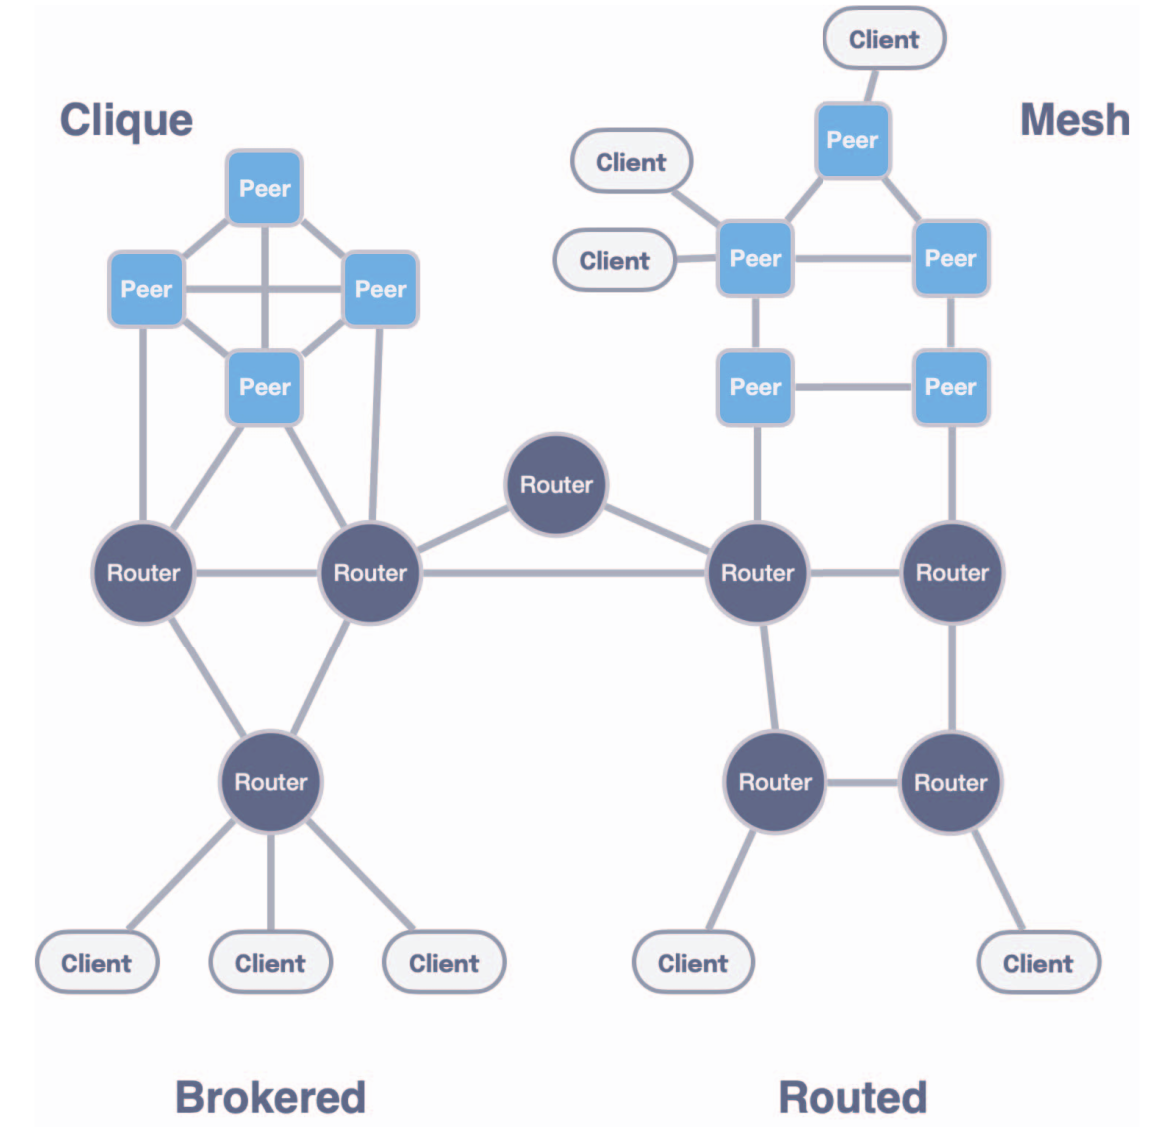
\includegraphics[width=.8\textwidth]{images/ch3/zenoh_networks.png}
  \caption{Possible network topologies in Zenoh \cite{corsaro_zenoh_2023}.}
  \label{fig:zenohnets}
\end{figure}

Finally, another positive aspect of Zenoh is that it is implemented with the additional goal in mind of having the lowest possible resource and memory footprint, which implies that it can run on a variety of different hardware platforms ranging from servers down to microcontrollers. For example, the control fields in its data packets can take up to as little as 5 bytes, as opposed to the at least 56 bytes required by the DDS. Moreover, it is almost completely agnostic of the underlying network layer, positioning itself in the protocol stack eventually as low as on top of the data link layer as showed in \Cref{fig:zenohstack}, thus supporting a wide variety of protocols and physical links including UART, Bluetooth, LoRa, Unix Sockets, TCP/IP, UDP/IP, QUIC, WebSockets, and CANbus, offering the same set of APIs and functionalities in all cases. Thanks to this level of versatility, Zenoh is a very good candidate to be used in the development of distributed autonomous systems, especially in those contexts where the DDS is not applicable due to the reasons discussed above, and it has already been successfully employed in industrial contexts achieving good performance in terms of both throughput and latency \cite{baldoni_facilitating_2021,greising_zenoh_2023} despite being relatively new, as its version \texttt{1.0} has been released in October 2024\footnote{\href{https://github.com/eclipse-zenoh/zenoh/releases/tag/1.0.0}{https://github.com/eclipse-zenoh/zenoh/releases/tag/1.0.0}}. For these reasons, it is included in the proposed architecture in its current state alongside some DDS implementations, to provide a complete set of communication tools that can be used in a variety of contexts, platforms, and applications.
\begin{figure}[t!]
  \centering
  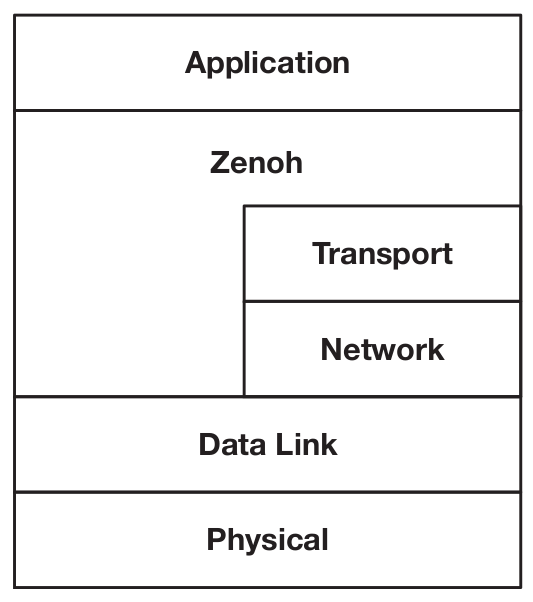
\includegraphics[width=.3\textwidth]{images/ch3/zenoh_stack.png}
  \caption{Placement of the Zenoh protocol in the network stack \cite{corsaro_zenoh_2023}.}
  \label{fig:zenohstack}
\end{figure}

\subsection{Robot Operating System 2}
\label{sec:ros2}
The previous sections presented a class of software solutions whose objectives align with those that emerge during the design of a distributed system, and aimed at providing real-time communication services. With all these elements in place, the next solution to be described is a middleware specifically designed for robotics applications, which are a particular case of distributed systems, and that is also widely employed in the industry and in the open-source community. Since autonomous robotics is one of the application settings for which the proposed architecture has been developed and in which it has been tested and employed, this particular middleware is of paramount importance for the rest of this work and will be described in the following in due detail.

\ROS \cite{macenski_robot_2022} is the second version of the \emph{Robot Operating System} middleware \cite{open_robotics_robot_nodate}, originally developed in 2007 by Willow Garage \cite{quigley_ros_2009}, a spin-off of the Stanford Artificial Intelligence Laboratory. Although its name might give a different idea, ROS is not an operating system in the traditional sense of process management and scheduling; rather, it started as a structured communications layer above the host operating systems of a heterogenous compute cluster. Then, ROS has evolved into a middleware that offers robotic and automation programmers services and APIs such as hardware abstraction, low-level device control, data exchange and inter-process communication, support for creating client-server modular architectures, and software package management. The entire project consists of a collection of software libraries and tools. It has always been open-source with a community-based development model and rigorous review processes: the source code of each version, ready for compilation and installation, is organized into various repositories hosted on GitHub, and documentation is published online alongside numerous \emph{design documents} that explain and comment on the design choices that are made and on the new features that are introduced. Fixes and innovations are tested in a \emph{Rolling} \cite{open_robotics_installation_nodate} release and subsequently introduced in stable releases, which follow an alphabetical naming scheme similar to that adopted by Canonical for the Linux distribution \emph{Ubuntu} \cite{canonical_ubuntu_nodate} and are thus often referred to as ``distributions''. Currently, the project is maintained and steered by the Open Source Robotics Foundation \cite{open_robotics_open_nodate}. Its open nature led to a steady increase in popularity over the years, and has contributed immensely to a worldwide renewal of the interest in robotics thanks to code sharing and open scientific contributions, both in a theoretical and in a practical sense, favoring the birth of a large number of communities, research projects, frameworks, laboratories and startups all over the world, sparking in the world of robotics a revolution similar to that happened in the software engineering world in the 90s with the advent of open-source software. Today if, \emph{e.g.}, a research team publishes a novel mapping algorithm for 3D LiDAR\footnote{Light Detection And Ranging, a class of sensors that use laser beams to reconstruct the depth of a scene and get a spatial reconstruction of the environment that surrounds them.} scans, it is very likely that the implementation of that algorithm will be made available as a ROS package, and that it will be tested and reviewed by the community, thus becoming a standard tool for all roboticists to use in their projects.
\begin{figure}[t!]
  \centering
  \includegraphics[width=.35\textwidth]{images/ch3/ros2logo.jpg}
  \caption{\ROS logo \cite{open_robotics_robot_nodate}.}
  \label{fig:ros2logo}
\end{figure}

By its documentation, \ROS supports the Linux, Windows, and macOS operating systems, but the reality is that support levels are defined by three \emph{tiers} that define support quality and frequency of updates. Currently, the only Tier 1 platform is Ubuntu Linux, in which a \ROS distribution can be installed either from binary packages or compiled from source; the latter installation technique can also be applied to different Linux distributions. As for Windows and especially macOS, since their closed nature with respect to Linux usually adds additional difficulties when developing robotic software, they are not so widely adopted and thus the community puts less effort into updating ROS for these platforms, also because of the lack of developers and testers that actually have these platforms available to develop on together with the expertise required to manage and integrate the whole ROS codebase.

For a summary of the history of ROS and an overview of its design goals, see \cite{gerkey_why_2014}. From that document, it is evident that the project soon proved potentially suitable for complex use cases, such as distributed and real-time management of collaborative swarms of robots or the homogeneous integration of different types of hardware and communication interfaces. A more technical and detailed description of the new features of the version 2, which introduces many of the most popular features, can be found in \cite{thomas_changes_2015}.

Historically, the first service offered by ROS was inter-process communication: in ROS 1, that was implemented by custom protocols built on top of TCP and UDP. The most significant difference between \ROS and the first version, and currently its greatest strength, is the fact that instead if reimplementing such protocols it sits directly above a layer, denoted as the RMW or ROSMiddleWare layer, which houses support for various communication middleware implementations aimed at distributed systems, such as the DDS and Zenoh. The first communication middleware to be integrated with ROS was the DDS \cite{woodall_ros_2014}: the entire middleware was indeed built on top of DDS, whose specific implementation is left to the user and is fully interchangeable, to implement the basic inter-process communication and data exchange services. This means that all the benefits of the DDS mentioned earlier such as ease of use and interface definition, Quality of Service, transmission configuration through discovery, and serialization, are immediately available to robotic system developers, solving quite a few problems but introducing new ones as previously discussed. Developers can also take advantage of ROS's standard libraries and the vast open-source ecosystem of packages based on ROS that are publicly available, as well as contribute their own work to advance the community of engineers and developers who use it.

From its origins, each version of ROS supports the following two programming languages: C++ and Python. This choice has been motivated by the high diffusion of both on nearly every platform, as well as by their intrinsic complementary nature. C++ is the most used and recommended for performance-critical as well as production applications, while Python is more suitable for rapid prototyping and for the development of scripts that interact with the system, as well as for high-level software modules that have no stric performance requirement but whose development and maintenance may benefit from a higher-level language. Moreover, Python is the de-facto standard programming language in contexts like machine learning and artificial intelligence, both fields that are having a disruptive impact on robotics. The \ROS project has also introduced support for other languages, such as Rust, Java, and plain C, and has developed a set of tools to facilitate the integration of these languages with the middleware, thus making it easier to develop software for robots using the language that best suits the task at hand. This is a significant improvement over the first version, which was limited to C++ and Python, and it is a clear sign of the project's commitment to keeping up with the times and the needs of the community.

To provide an idea of the main services offered by this middleware relevant to this work, the key features of \ROS will now be described following a top-down approach, eventually reviewing some auxiliary but very useful tools and frameworks; thus, many minor utilities are excluded for the sake of clarity but readers are referred to the technical documentation \cite{open_robotics_ros_nodate} and basic tutorials \cite{open_robotics_tutorials_nodate} for these aspects.

\subsubsection{Build system}
\label{sec:ros2_buildsys}
In the ROS ecosystem as in many similar contexts, software is naturally divided into units called \emph{packages}. The idea is that each package constitutes a standalone software module, designed to fulfill a specific function within the system's overall architecture, potentially interacting with others at various levels and using specific services offered by the system itself through APIs or specialized hardware. Nevertheless, as has been highlighted several times, a robot presents a different scenario from those typical of software development and it is not uncommon for a developer to work on multiple packages simultaneously. Adding to this complexity is the fact that if different modules need to interact, their corresponding packages will inevitably be interdependent. Therefore, a common system is needed to simplify the creation of a \emph{workspace} in which to develop, execute and test the software contained in multiple packages. The solution provided by \ROS consists of a universal build system applicable to any context where this middleware is employed and divided into two modules, with the reasons for this approach described in \cite{thomas_universal_2017}.

Initially, there is \emph{colcon} \cite{thomas_colcon_nodate}. It was originally intended to be a tool that automates and simplifies the compilation and installation of Python or C++ code packages via CMake\footnote{CMake \cite{kitware_cmake_nodate} is a cross-platform free software for build automation, whose name stands for ``cross-platform \texttt{make}.'' It was developed to simplify the build process by providing a scripting language to easily automate it entirely even for complex projects.} \cite{kitware_cmake_nodate} or Setuptools \cite{eby_setuptools_nodate} for use with \ROS, but soon it became a more general project of its author. Today, it is used even outside of the robotics world to manage large projects and codebases: it is not uncommon to find software libraries and tools whose source code can be managed and built using colcon. \ROS relies on colcon to organize every aspect of a workspace, intended as a collection of packages either in source code or binary\footnote{In this context, the term \emph{binary} identifies a way in which software can be shipped which does not include source code files, and is instead limited to compilation output in the form of either libraries to link against or executables to run.} form. Essentially, colcon creates a workspace by defining some basic directories in the file system where both source code and build artifacts will reside, and then manages compilation and installation according to either automatic or specified rules resolving dependencies automatically, \emph{i.e.}, ensuring that all external pieces of software that are required are actually present on the system and correctly configured. Each package, to be manageable by colcon, must include a \emph{package manifest} in the form of an XML file\footnote{eXtensible Markup Language, based on a syntactic mechanism that allows the definition and control of the meaning of elements contained within a document or text. It is used in web pages or for collecting data in a text file so that it is also interpretable by a computer program: parsing can be easily performed using appropriate libraries.} in which all the characteristics of a software module, such as its name or dependencies, are listed. Installation may result in the generation of an executable file or a shared library, and possibly also of symbolic links to a location within the workspace where builds are performed; this greatly simplifies matters when testing the software and compiling it multiple times, as it avoids having to modify the installation points each time, always pointing to the latest executable or configuration file. The many command-line options of colcon also allow interaction, if necessary, with lower-level tools used at various stages of compilation and build.

In addition to the typical challenges related to building interdependent packages, it is also necessary to address those concerning integration with preexisting libraries and interfaces that compose a \ROS installation. To address this and many other issues, the second module is used: \emph{ament} \cite{thomas_build_2015}. It is a collection of Python scripts invoked automatically by colcon that complete the build process by resolving dependencies with other \ROS packages and ensure that paths, environment variables and scripts are correctly set up, so that the software can later be executed without issues and with a minimal set of commands being necessary. This system proves effective: when having multiple packages in a workspace, they can all be built together with a single command. Compare this ease of use and the integration of new solutions like CMake and Setuptools with, \emph{e.g.}, the \texttt{make}-only build system of MARTe2 discussed in \Cref{sec:related_work_marte2} and you may start to get an idea of the advantages of using \ROS in a complex software project for a distributed autonomous system.

\subsubsection{Interfaces}
\label{sec:ros2_interfaces}
In \ROS, like in the DDS, it is possible to specify the format of the data packets exchanged among software modules, which are called \emph{messages}, using special text files called \emph{interface files} \cite{thomas_interface_2019}. In these files, similarly to DDS IDL files, the structure of the packet is defined by specifying each field on a separate line by a name and a data type. Data types range from integers or floating-point numbers to strings, and even variable-length arrays. It is considered good practice to group these files into packages consisting solely of interface definitions, which are then built and installed using the same build system: the result in this case is a collection of Python classes, and C++ header files and shared libraries that define the types of the data packets as well as the serialization and deserialization operations, which can then be included and linked in other modules that need to exchange data in such formats. In practice, a \ROS developer never needs to concern themselves with anything related to format specification, serialization, transmission, reception, or deserialization: all of this is automatically managed by \ROS via its RMW layer.

Unlike a standard DDS, however, \ROS also allows other two communication primitives, each with its own interface file format, which extend the communication services offered beyond the classic publish-subscribe paradigm. The communication primitives are:
\begin{itemize}
  \item \textbf{Messages}: they are the most common and are used to exchange data packets among software modules in a publish-subscribe fashion; they are specified in \texttt{.msg} files. An illustrative scheme is provided in \Cref{fig:ros2msg}, and the definition of the \texttt{Image} message from the \texttt{std\_msgs} library is provided as an example in \Cref{lst:imagemsg}.
  \item \textbf{Services}: they are used to request a computation to be performed by another software module and to receive the result, enabling a client-server, \emph{stateless} communication; they are specified in \texttt{.srv} files. Note that in this context, the term \emph{stateless} identifies a kind of communication that has no intermediate states between its beginning and end: in a service call, a \emph{client} requests a computation to the \emph{server}, which performs it and returns the result to the client, wihtout any further interaction between the two being possible and usually in a short time. This is useful for simple transmissions like quick parameter setting or data retrieval, but not for complex interactions that require multiple steps, long computation times, or many possible outcomes. An illustrative scheme is provided in \Cref{fig:ros2srv}, and the definition of the \texttt{AddTwoInts} service, which allows to perform the addition between two integers and is widely employed in tutorials, is provided as an example in \Cref{lst:addtwointssrv}: note how the two request and result messages are delimited in the file by the three dashes.
  \item \textbf{Actions}: they are used to request a computation to be performed by another software module and to receive the result, enabling a client-server, \emph{stateful} communication; they are specified in \texttt{.action} files. In this context, the term \emph{stateful} identifies a kind of communication that has intermediate states between its beginning and end: in an action call, a \emph{client} requests a computation to the \emph{server}, which performs it and returns the result to the client, but the server can also send feedback to the client during the computation, and the client may even request the cancellation of the ongoing operation to the server. Moreover, the server may reply to the client at the end of the operation sending back two items: the actual output value of the computation, if any, and various codes that describe nearly any possible outcome. This is the most flexible and powerful communication primitive offered by \ROS, usually employed in software modules that perform complex operations like navigation or tracking, where the client needs to know the status of the computation and possibly to interact with the server during its execution. An illustrative scheme is provided in \Cref{fig:ros2act}, the state machine of an action goal is portrayed in \Cref{fig:ros2goalfsm}, and the definition of the \texttt{Fibonacci} action, which in many tutorials expresses the computation of the Fibonacci sequence up to a given order, is provided as an example in \Cref{lst:fibonacciact}: note how the three request, result, and feedback messages are again delimited in the file by the three dashes.
\end{itemize}
All of these are implemented on top of the RMW layer. In the case of DDS, they are all implemented using topics: a service maps to two topics, one for the request and one for the reply, while an action is implemented with two services: the \emph{goal service} to place the request for a computation and the \emph{result service} to request its output, and a \emph{feedback topic}. In the case of other middleware that natively supports client-server communication, like Zenoh, the implementation is more straightforward and efficient, as the middleware itself manages the stateful communication and the client-server interaction, thus reducing the overhead and the complexity of the system.
\begin{figure}[t!]
  \centering
  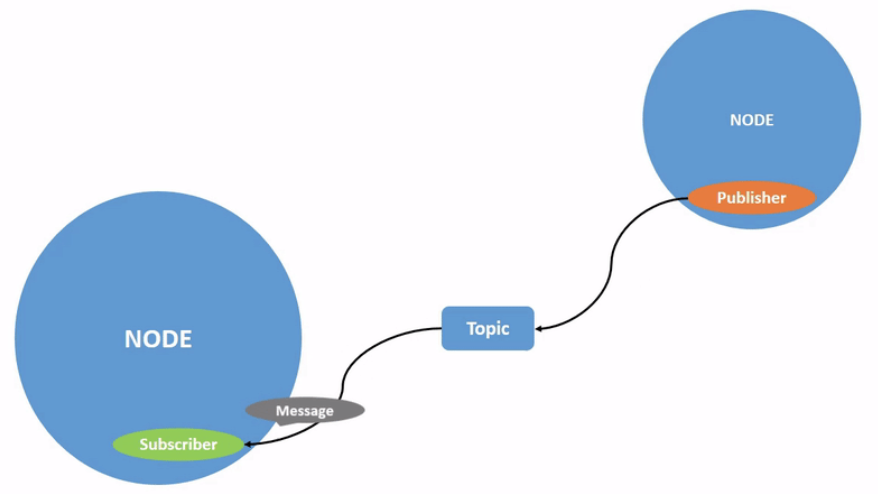
\includegraphics[width=.6\textwidth]{images/ch3/ros2Msg.png}
  \caption{Scheme of the message communication primitive \cite{open_robotics_understanding_nodate}.}
  \label{fig:ros2msg}
\end{figure}
\begin{figure}[t!]
  \centering
  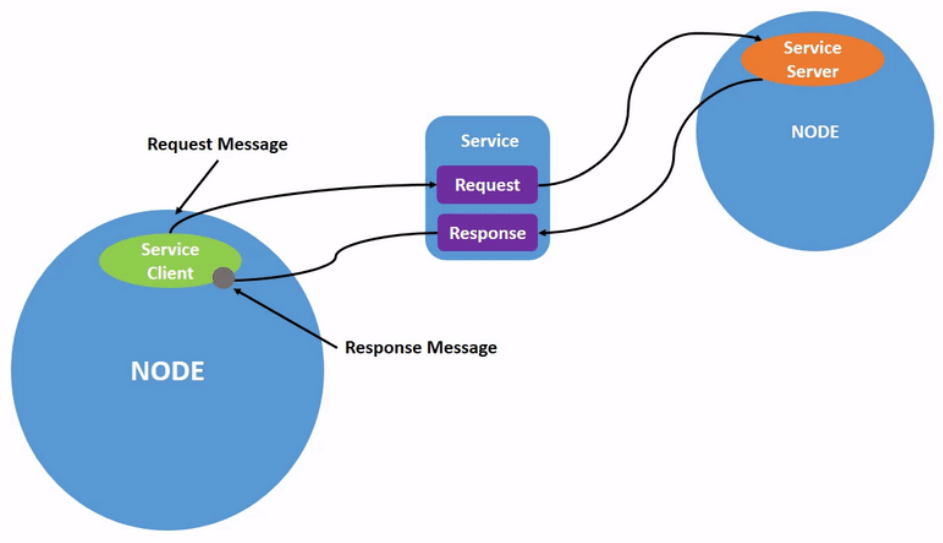
\includegraphics[width=.6\textwidth]{images/ch3/ros2Srv.png}
  \caption{Scheme of the service communication primitive \cite{open_robotics_understanding_nodate-1}.}
  \label{fig:ros2srv}
\end{figure}

\newpage
\begin{center}
\begin{minipage}[t]{.9\textwidth}
\begin{lstlisting}[caption=Definition of the \texttt{sensor\_msgs/Image} message., label={lst:imagemsg}]
# This message contains an uncompressed image
# (0, 0) is at top-left corner of image

Header header # Header timestamp should be acquisition time of image
              # Header frame_id should be optical frame of camera
              # origin of frame should be optical center of camera
              # +x should point to the right in the image
              # +y should point down in the image
              # +z should point into to plane of the image
              # If the frame_id here and the frame_id of the CameraInfo
              # message associated with the image conflict
              # the behavior is undefined

uint32 height # image height, that is, number of rows
uint32 width  # image width, that is, number of columns

string encoding # Encoding of pixels -- channel meaning, ordering, size
                # Taken from the list of strings in
                # include/sensor_msgs/image_encodings.h

uint8 is_bigendian # Is this data big-endian?
uint32 step        # Full row length in bytes
uint8[] data       # Actual matrix data, size is (step * rows)
\end{lstlisting}
\end{minipage}
\end{center}

\begin{figure}[t!]
  \centering
  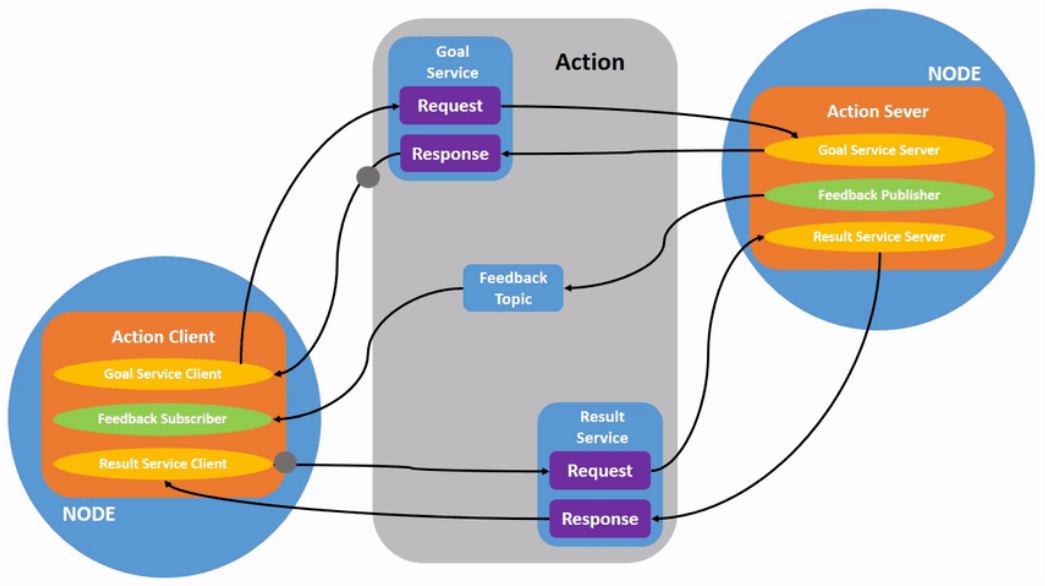
\includegraphics[width=.6\textwidth]{images/ch3/ros2Act.png}
  \caption{Scheme of the action communication primitive \cite{open_robotics_understanding_nodate-2}.}
  \label{fig:ros2act}
\end{figure}
\begin{figure}[t!]
  \centering
  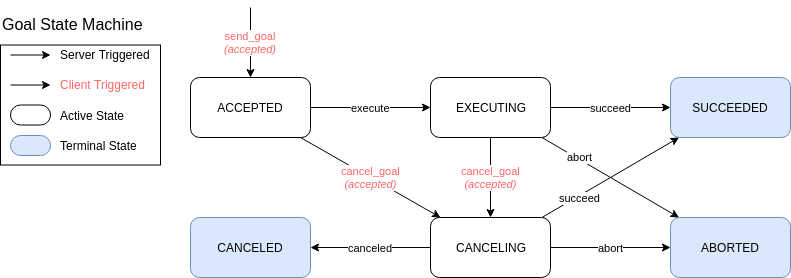
\includegraphics[width=.8\textwidth]{images/ch3/goalStateMachine.png}
  \caption{State machine of an action goal \cite{biggs_actions_nodate}.}
  \label{fig:ros2goalfsm}
\end{figure}

\newpage
\begin{center}
\begin{minipage}[t]{.9\textwidth}
\begin{lstlisting}[caption=Definition of the \texttt{example\_interfaces/AddTwoInts} service., label={lst:addtwointssrv}]
int64 a
int64 b
---
int64 sum # = a + b
\end{lstlisting}
\begin{lstlisting}[caption=Definition of the \texttt{example\_interfaces/Fibonacci} action., label={lst:fibonacciact}]
# Goal
int32 order
---
# Result
int32[] sequence # Variable-length array of 32-bit integers
---
# Feedback
int32[] sequence # Variable-length array of 32-bit integers
\end{lstlisting}
\end{minipage}
\end{center}

\subsubsection{Core API organization}
\label{sec:ros2_coreapi}
To give an idea of how an architecture based on ROS for a distributed autonomous system may work, it is instrumental to present briefly the organization of the core API of \ROS, which is shown in \Cref{fig:ros2coreapi}. The core API is the set of libraries and tools that implement the basic functionalities offered by the \ROS middleware, intuitively starting from the communication layer and going up to the services offered to the application layer. Below the core API lies the communication middleware layer, which hosts the selected implementation(s) of the communication  middleware(s) to employ; such implementations, when made available to the open-source community, are usually shipped together with \ROS base packages. This layer is represented in \Cref{fig:ros2coreapi} by the blue blocks at the bottom. On top of it all, there are code and applications that use the services offered by \ROS and everything else above them: these levels are represented by the top gray block in \Cref{fig:ros2coreapi}. The core API, laying in the middle, is divided into several modules, each of which is responsible for a specific aspect of the \ROS middleware. The most important levels are, from top to bottom:
\begin{itemize}
  \item \texttt{rmw} \textbf{level}: the ROSMiddleWare level hosts a set of C libraries that abstract different implementations of communication middlewares like, \emph{e.g.}, many DDS implementations and Zenoh, offering a common interface to upper levels to achieve basic communication functionalities.
  \item \texttt{rcl} \textbf{level}: the ROS Client Support Library level hosts a C library that implements basic entities like \emph{nodes}, discussed in \Cref{sec:ros2_nodes}, \emph{publishers} and \emph{subscribers}, service and action \emph{clients} and \emph{servers}, and \emph{timers}.
  \item \textbf{ROS Client Library level}: at this level, various libraries are implemented to offer support for programming languages other than C, like Python and C++. The entities defined in the lower levels are extended here, adding language-specific features and abstractions. Moreover, another core entity is defined at this level: the \emph{executor}, which manages the execution of ROS-related jobs in dedicated OS threads, discussed in \Cref{sec:ros2_nodes}.
\end{itemize}
\begin{figure}[t!]
  \centering
  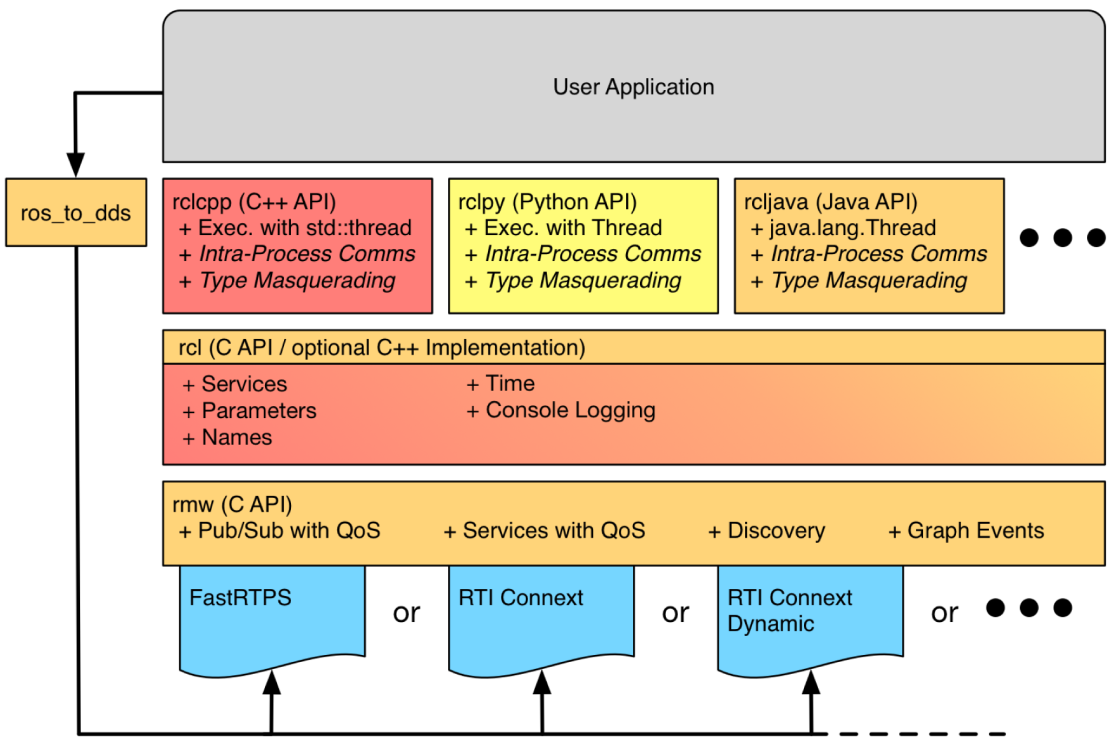
\includegraphics[width=.8\textwidth]{images/ch3/ros2_stack.png}
  \caption{Core \ROS API organization \cite{macenski_impact_2023}.}
  \label{fig:ros2coreapi}
\end{figure}

\subsubsection{Nodes and executors}
\label{sec:ros2_nodes}
In \ROS applications, the most important entity is the \emph{node}. Conceptually, a \ROS node is an operational unit of the distributed system, capable of performing a specific task for which it has been designed. In the code, irregardless of the programming language employed, a \ROS node is an object of a class, that usually expands the base \texttt{Node} class of the specific client library used, adding features that are specific for the operations that the node has to perform. Primarily, and thanks to class members and methods they inherit, nodes act as access points towards the middleware that enable application code to use \ROS features. For example, a node can create publishers and subscribers to exchange messages, service servers or clients, and even action servers and clients. Nodes have \emph{parameters}, which are variables that can be set from the outside to configure the behavior of the node using a very versatile API: a node parameter is identified by a name and a type, and can be set at the startup of the node or at run time; in the context of an autonomous robot, a \ROS node parameter may be, \emph{e.g.}, a gain for a control law being applied to the underlying physical system. Parameters can be queried and updated from both users and other software modules, \emph{i.e.}, other nodes in the architecture, possibly deployed on different hosts in a distributed fashion.

The main idea is always that, to describe and design a distributed system, the node is a unit that performs computations that are aimed at performing a specific task, implementing a specific subsystem of the overall architecture. To achieve this, and to fully comply with the distributed paradigm even in real-time contexts, nodes generate computational \emph{jobs} when specific events occur. Such events must be handled accordingly, in a way that is orchestrated by the middleware. The situation at hand is described in \Cref{fig:ros2exec}, which shows the event-based execution model of \ROS. In this model, aside from synchronous computations that are part of the user code, part of the processing is handled asynchronously when the following specific events occur:
\begin{itemize}
  \item a subscriber receives one or more messages;
  \item a timer expires;
  \item a service request is received;
  \item an action goal or result request is received;
  \item a parameter is updated.
\end{itemize}
Apart from timers, the parameter subsystem is implemented using services which map to topics together with actions, but for the sake of clarity \Cref{fig:ros2exec} highlights the most important event groups. Each of those can be processed by a user-specified callback, that is registered as part of the node configuration. Then, nodes carrying their asynchronous workload are added to an executor, which handles callbacks in groups over one or more OS thread; node that executors can handle multiple nodes at the same time. To set things in motion, hence the name, in any \ROS application the executor is then started by calling its \texttt{spin} method.
\begin{figure}[t!]
  \centering
  \includesvg[width=.8\textwidth]{images/ch3/ROS2_executor_scheme.svg}
  \caption{\ROS event-based execution model.}
  \label{fig:ros2exec}
\end{figure}

Over the years, the real-world performance of this paradigm has been thoroughly evaluated \cite{bedard_message_2023,maruyama_exploring_2016,puck_distributed_2020,kronauer_latency_2021}. What emerged, especially in the early versions of the framework, is that although conceptually correct it was affected by some design flaws. First of all, while in its ideal contexts the DDS performs well with little to no real-time overheads, the RMW abstraction could introduce some unwanted latencies. Moreover, the \ROS executor, which is the entity that manages the execution of the asynchronous jobs, was not designed to be real-time capable: its algorithm lacks any notion of priority and it seems to favor timers over any other kind of event, to empirically maximize responsiveness. If one thinks that commercial robots with ROS stacks are not only available but employed in the industry since almost a decade, it is clear that the \ROS executor is not a showstopper: in many contexts, things work fine because that level of strict real-time requirements is not needed, and as long as the system resources are not saturated both throughput and latencies remain acceptable even with such primitive algorithms. Nonetheless, the community has got the message: many solutions to these issues have been put in place and the core \ROS libraries listed in \Cref{sec:ros2_coreapi} are constantly updated and improved. The interested reader can find references to some of these solutions in \cite{bedard_message_2023}, while a novel priority-based executor suited for real-time applications is presented in \cite{staschulat_rclc_2020}. Finally, problems induced by the DDS, as discussed in \Cref{sec:zenoh}, are addressed by the ongoing adoption of Zenoh as a communication middleware in \ROS \cite{open_robotics_ros_2023}, which is expected to be completed in the next few years. Another solution that deserves a mention is the \emph{node composition} \cite{macenski_impact_2023}, which is similar to the way in which software modules are handled in the MARTe2 framework presented in \Cref{sec:related_work_marte2}. In \ROS, C++ nodes can be compiled in two ways: either as parts of executables or as standalone shared libraries\footnote{A shared library is a collection of compiled functions and routines that can be used by multiple programs simultaneously, allowing for code reuse, efficient memory usage, and simpler software updates by sharing a single copy of the library in memory at runtime.}, denoted as \emph{components}. Components can either be loaded and unloaded at run time, inside a process that hosts executors for their jobs acting as a \emph{component container}, or they can be statically linked to an executable. The thing is that, in either of these ways, multiple nodes end up running inside the same process, thus sharing the same memory and address space. This allows to avoid the overhead of inter-process communication, completely bypassing the RMW layer and anything underneath, leading to very low latencies and high throughput. This is a very powerful feature that can be used to implement complex systems in an efficient way, as demonstrated in \cite{macenski_impact_2023}, provided that nodes are stable enough to run in the same process: in case one of them crashes, the whole process will be terminated, and all the other nodes will be stopped. This is a trade-off that must be carefully evaluated when designing a distributed system based on \ROS, and the usual way of running each node in its own process remains the suggested one for the early stages of development and testing.

\subsubsection{Launch system}
\label{sec:ros2_launch}
A \ROS executable, or a group of such, must be launched using specific middleware commands to ensure that all necessary daemons and logging subsystems are activated. The middleware subsystem responsible for this is called the \emph{launch system}, and the action of starting up multiple modules composing an architecture is called \emph{launching}.

There are two ways to launch modules: either by using command-line tools to start each module individually, or by running scripts that specify the whole set of modules to run, together with their parameters and configuration options. These scripts are called \emph{launch files}, and they are usually added as part of any package that contains executable code, and to any architecture once all the modules have been collected, to boot everything up with a single command. A launch file specifies, according to their format \cite{open_robotics_launch_nodate}, the configuration with which the executable should be launched, including details ranging from input arguments to how logging should be managed, either in the console or in files, or both. Unless specified otherwise, any log files generated by the process output will be saved in a standard path, typically a subdirectory of the home directory (\emph{e.g.}, \texttt{$\sim$/.ros/} on Linux).

\subsubsection{Data recording and playback}
\label{sec:ros2_bags}
For various purposes, such as testing or post-analysis, it may be necessary to capture all the messages that were handled by the middleware during a specific time interval and on particular topics. \ROS provides this service through a system called \emph{bagging} \cite{open_robotics_recording_nodate}: using specific commands, it is possible to record messages sent on certain topics into a file, with configurable format and compression algorithms. This file, which also includes information about the message interfaces it contains, can be processed by other software to review the data. Bags can also be replayed from the beginning using another command, which creates ad-hoc publishers that will re-publish the recorded messages at an original or user-defined rate. This way, it is possible to develop, test, debug, and even tune algorithms offline, without the need to perform an experiment with the actual robot each time, just by replaying the recorded data, avoiding potentially risky or costly operations. This feature is so popular that the vendors of many proprietary scientific software like, \emph{e.g.}, MATLAB \cite{mathworks_matlab_nodate} or LabVIEW \cite{national_instruments_labview_nodate}, have developed plugins to read and write \ROS bags, and many open-source tools have been developed to parse and process them, some of which are part of the \ROS ecosystem themselves.

\subsubsection{Visualization and simulation}
\label{sec:ros2_sim}
A complete installation of \ROS includes several useful tools for debugging, such as commands for inspecting active topics, examining their interfaces, measuring the publication rate, and launching publishers as needed. There are also software tools that are not required for the operation of a robot and, in fact, are superfluous in that context but extremely useful during the development phase. It is appropriate to mention at least the following:
\begin{itemize}
  \item \textbf{Gazebo} \cite{open_robotics_gazebo_nodate}: this is an open-source simulator natively compatible with ROS, capable of interacting with middleware topics to send and receive data. It allows for the creation of 3D models of robots—complete with sensors and actuators—as well as the environments in which they operate, using XML-based syntax, and provides a platform to test control and perception algorithms. Gazebo offers a 3D visualization of the simulated world, and it can be used to simulate the behavior of a robot in a virtual environment thanks to its embedded real-time physics engine. Moreover, thanks to its open-source nature, Gazebo can be extended with plugins that add new features or modify existing ones, like implement simulated sensors and scenario elements, and it can be integrated with other software tools like MATLAB \cite{mathworks_matlab_nodate}, Simulink \cite{mathworks_simulink_nodate}, or LabVIEW \cite{national_instruments_labview_nodate}.
  \item \textbf{RViz} \cite{open_robotics_rviz_nodate}: this is a 3D visualization tool that can be used to display the state of a robot and its environment, as well as the data that is exchanged among the various modules of the system. It is a very useful tool for debugging and testing, as it allows to visualize the data that the robot is processing in a way that is easy to understand, and to interact with the system by sending commands and receiving feedback. RViz can be used to display the robot's position and orientation, the data from its sensors, the map of the environment, and the planned path, among other things. It can also be used to display the data exchanged among the various modules of the system, like the messages sent on the topics, the services called, and the actions performed. RViz can be used to visualize the data in 3D, 2D, or even in a tabular form, and it can be configured to display only the data that is relevant to the task at hand. As Gazebo, it is open-source and extensible with plugins that users can develop themselves.
\end{itemize}
An example of the capabilities of these two tools together is shown in \Cref{fig:ros2rviz}.
\begin{figure}[t!]
  \centering
  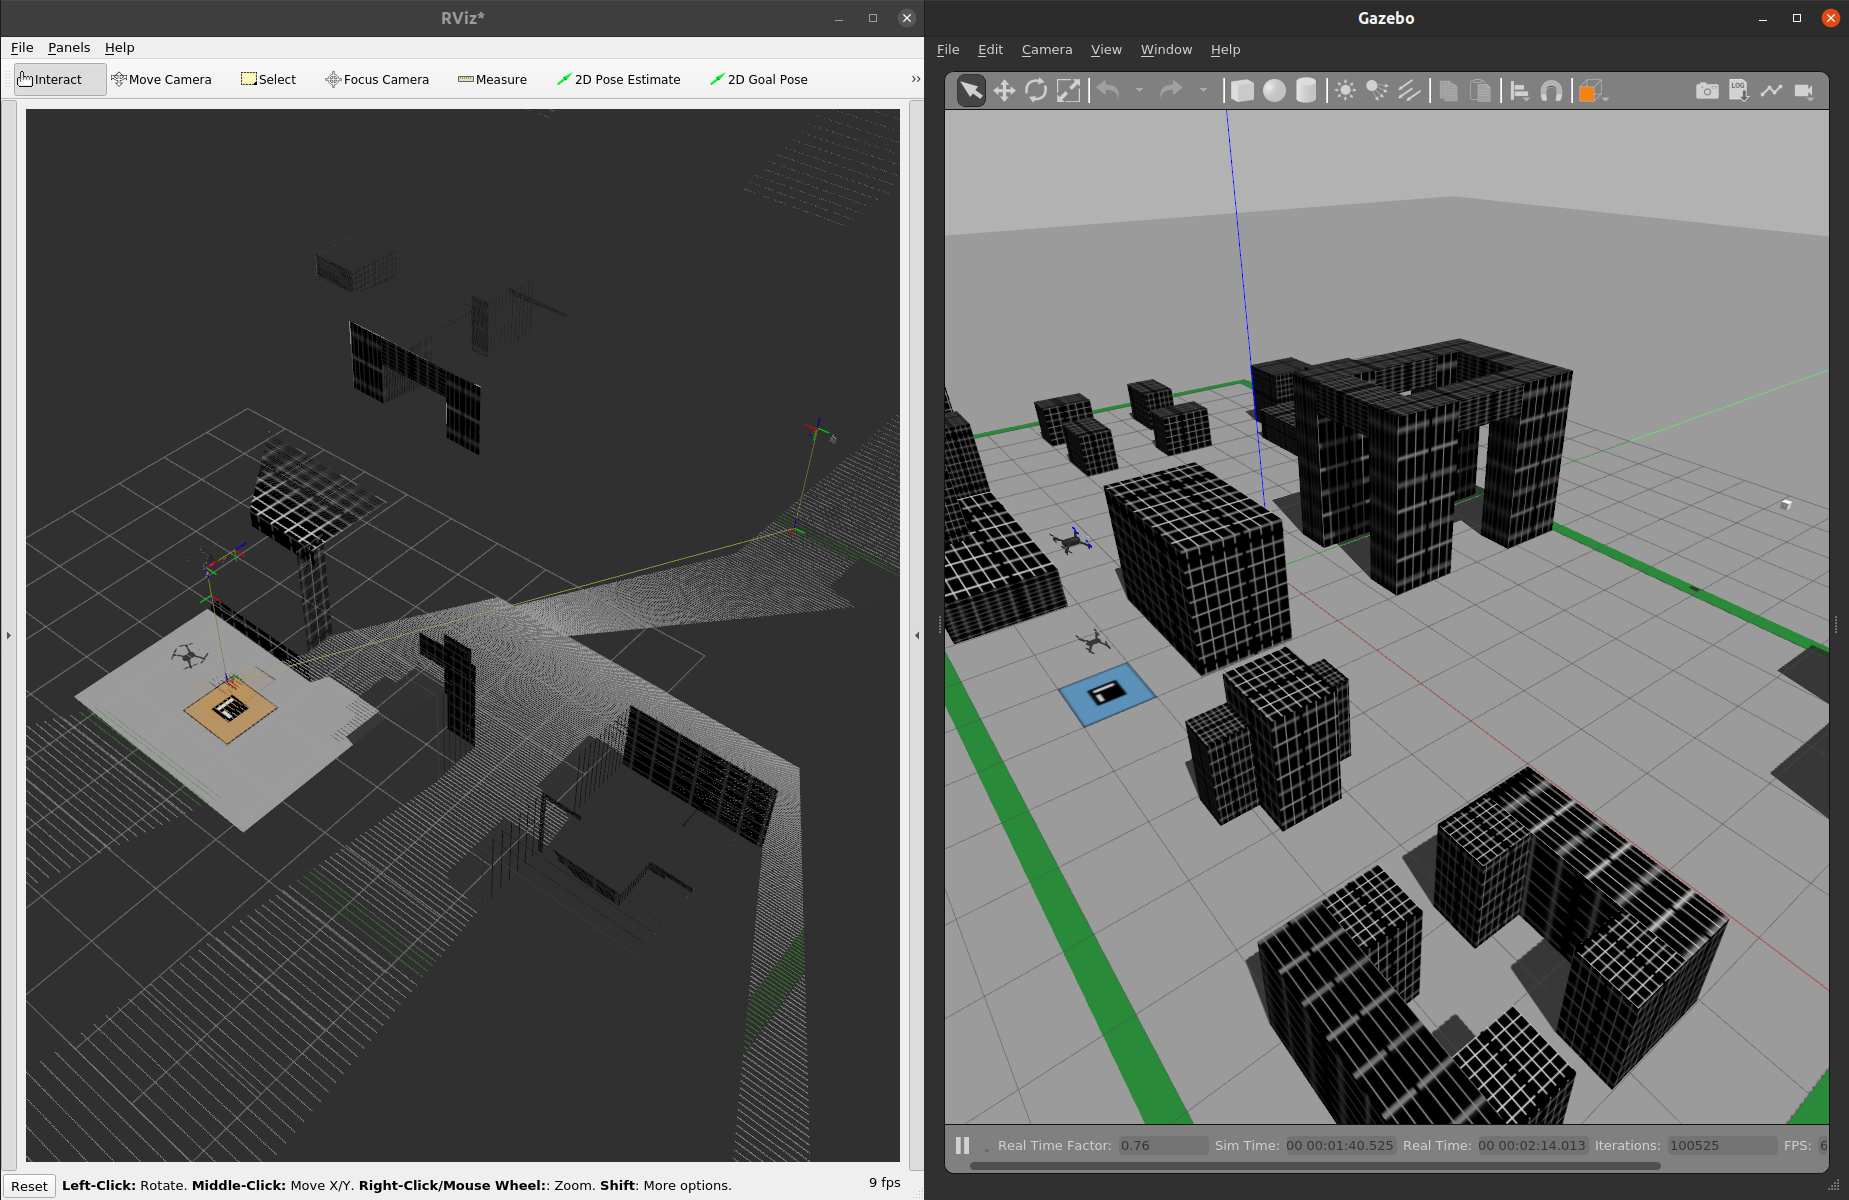
\includegraphics[width=.9\textwidth]{images/ch3/ros2simulation.png}
  \caption{Simulation of an autonomous drone with imaging and depth sensors in Gazebo (right) and visualization of the data in RViz (left).}
  \label{fig:ros2rviz}
\end{figure}

\subsubsection{Applications and related frameworks}
\label{sec:ros2_app}
The previous sections highlighted the main features of the Robot Operating System 2 middleware, aimed at the development and organization of software for distributed autonomous robotic systems. The \ROS ecosystem is vast and varied, and it is used in many different application areas, from industrial automation to service robotics, from autonomous vehicles to drones, from medical robotics to space exploration. The \ROS middleware is also used in many research projects, both in academia and in industry, and it is the basis for many open-source software libraries and tools that are widely used in the robotics community. Its features, discussed so far, clearly defined its relevance in the context of the present work, and it will be included in the proposed architecture as illustrated in the following chapters. To conclude the presentation of \ROS, some further references are in order to clarify its diffusion in both the research and industrial communities, as well as the variety of projects that are based on it.

One of the areas in which ROS has historically been employed the most is that of mobile, terrestrial robotics. In this field, there are a variety of problems to solve, ranging from localization to mapping, from path planning to obstacle avoidance, from perception to manipulation. One of the most famous projects related to this setting is Nav2 \cite{open_navigation_nav2_nodate,macenski_desks_2023,macenski_marathon_2020,macenski_regulated_2023,merzlyakov_comparison_2021}, the official ROS navigation stack for mobile robots. This package, originally developed to expose APIs for autonomous movement of mobile, planar robots, has evolved into a vast framework covering nearly every aspect of autonomous navigation: environment mapping and reconstruction, path planning and smoothing, obstacle avoidance, localization, and even human-robot interaction. A variety of algorithms for each case is available, and the system is designed to be modular and extensible in each of its parts, including visualization plugins for RViz and simulation elements for Gazebo. Operations carried out by the many modules of the framework are orchestrated by automata such as behavior trees \cite{iovino_survey_2022}.

Another area that robots revolutionized is that of industrial automation, in which manipulators of different sizes and shapes are employed to perform repetitive tasks with high precision and reliability. In this context, \ROS is used to control the robots and to interface them with other systems, like sensors and actuators, and to manage the data that is exchanged among them. One of the most famous projects in this field is MoveIt \cite{picknik_robotics_moveit_nodate,gorner_moveit_2019,coleman_reducing_2014,bonci_robot_2023}, the official ROS manipulation stack for industrial robots. As Nav2 for mobile robotics, MoveIt is very large in terms of functionalities it offers, all of which are built on \ROS tools and libraries. First, it allows the developer to define a physical and kinematic model of the robot using the Unified Robot Description Format (URDF), which is a particular kind of XML file in which the geometrical and dynamic properties of a robot can be specified: masses, inertias, joints, links, and even sensors. Then, it provides extensible software modules to interface with the robot hardware, which is usually made of custom microcontrollers with their own communication protocols and semantics. Finally, it allows the specification of states and movement operations thanks to many path planning and tracking algorithms, and it offers plugins for the RViz visualizer to turn it into a Graphical User Interface (GUI) for the robot.

One setting which is still relatively young is that of aerial robotics. Autonomous drones and aircraft can be used in a variety of applications thanks to their ability to fly, from surveillance to search and rescue, from agriculture to entertainment. The capabilities of the \ROS framework in this context are still being explored by the robotics community, particularly because a flying platform is more complex to control than a terrestrial one, and because the environment in which it operates is more dynamic and less predictable. Some preliminary results by the author, which led to the development of this work and can be considered its embryonic stage, are presented in \cite{bianchi_novel_2023,bianchi_efficient_2023}.

Finally, it is important to asses the kind of hardware platforms on which \ROS has been designed to run. If one recalls the discussions held in the previous sections, it appers clear that the lowest tier of hardware on which \ROS-based software can run is a Single-Board Computer (SBC), which is usually the highest grade of hardware that can be found on autonomous robots. However, as previously remarked, robots are complex systems that usually also include specialized hardware like microcontrollers to drive both sensors and actuators. It would be desirable to be able to organize the code for such devices in a similar way to that based on \ROS, even leveraging similar communication paradigms and abstractions. This is where the micro-ROS project \cite{eprosima_micro-ros_nodate} comes into play. Developed by eProsima, one of the major developers of DDS implementations as well as one of the greatest contributors to the \ROS codebase, micro-ROS is a reduced software stack implemented mostly in C, which offers a subset of the core \ROS functionalities with a minimal memory footprint and computational overhead. Its software stack, shown in \Cref{fig:microrosstack}, is designed to run on a variety of Real-Time Operating Systems (RTOS) supporting their task scheduling and memory allocation APIs, and it is developed to preallocate or statically allocate memory to avoid dynamic memory allocation and deallocation, which is a common source of bugs and performance issues in real-time systems. The micro-ROS stack is designed to be used in conjunction with the full \ROS stack, exchanging data over topics in both directions thanks to a bridge put in place by the Micro XRCE-DDS \cite{eprosima_micro_nodate} implementation, composed by an agent application running on a PC or SBC which talks with a client running on the microcontroller. Supported physical links include Ethernet, Wi-Fi, and even serial connections. As every solution presented up to this point, micro-ROS is open-source and its community is growing rapidly, as is the number of experimental evaluations, projects, and supported microcontrollers like, \emph{e.g.}, the STM32 series from STMicroelectronics \cite{stmicroelectronics_stm32_nodate} or the ESP32 series from Espressif Systems \cite{espressif_systems_esp32_nodate}.
\begin{figure}[t!]
  \centering
  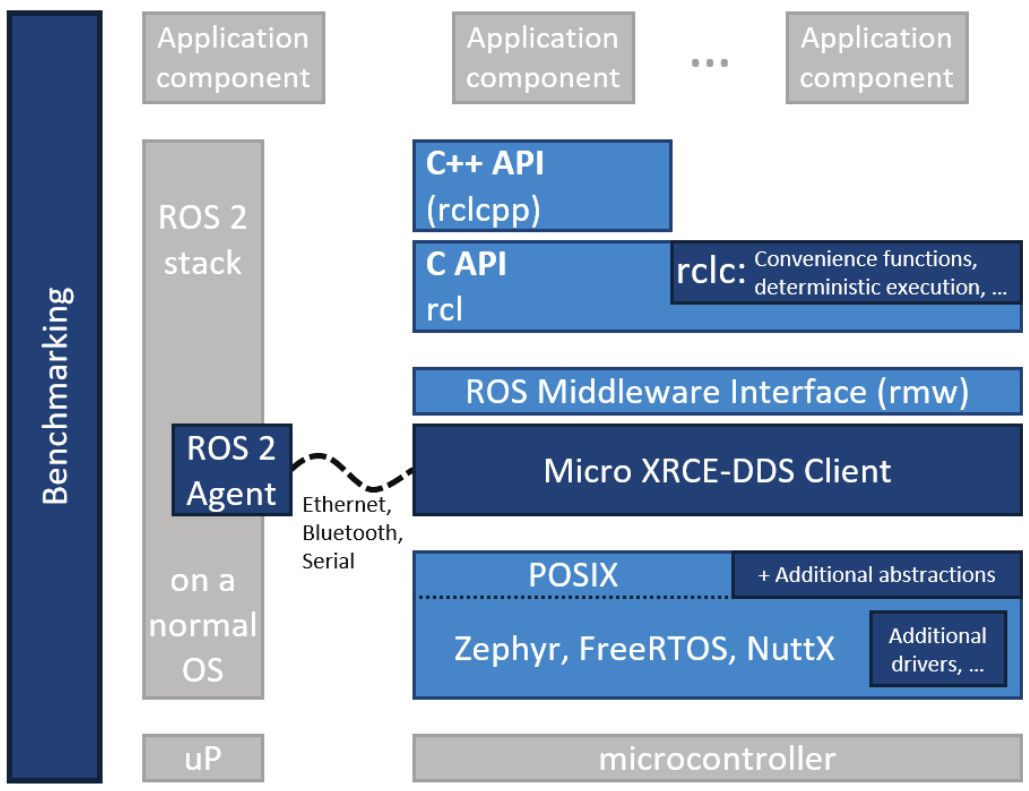
\includegraphics[width=.8\textwidth]{images/ch3/microros_stack.png}
  \caption{micro-ROS architecture \cite{eprosima_micro-ros_nodate}.}
  \label{fig:microrosstack}
\end{figure}

\section{Containerization}
\label{sec:containerization}
Recalling the Modularity (M) requirement, suppose that a software module requires external dependencies, \emph{e.g.}, libraries or tools to be built and run. These external dependencies may not be made part of the module sources but have to be set up in the systems that host it. Setting up a development and execution environment addressing situations like this is a common but usually also quite complex task. Multiplying the complexities by the number of different hardware platforms that the software module has to run on, one may get a set of problems that are hard to manage. This is the motivation of the Abstraction (A) requirement: the architecture should provide a way to abstract the software modules from the hardware platforms they run on, to allow one to develop software that is portable across different platforms and to simplify the setup of the development and execution environments. Historically, the technology that allowed this kind of abstraction is called \emph{virtualization}, which in general comes at the price of a significant overhead in terms of computational resources and performance. Preventing this is the reason why, in \Cref{sec:prb_requirements}, the Overhead (O) requirement is also stated, which requires the architecture to be as lightweight as possible to avoid any unnecessary computational overheads that may affect the performance of the software modules. The technology that addresses all these requirements, forming a base layer of the proposed architecture, is called \emph{containerization}.

Containerization represents a transformative approach to software deployment that addresses fundamental challenges in application portability and environmental consistency \cite{pahl_cloud_2019}, while remaining distinct from traditional virtualization technologies \cite{dua_virtualization_2014}. While virtualization employs hypervisors to create virtual machines with independent operating systems, containerization achieves isolation by leveraging the host operating system kernel to establish separate environments that share the underlying OS. This architectural difference results in containers exhibiting substantially lower overhead compared to virtual machines, enabling higher resource density and improved efficiency. The technology effectively resolves the challenges of inconsistent behavior across deployment environments by bundling applications with their dependencies, ensuring uniform operation across diverse platforms. This capability proves particularly valuable in distributed software architectures where deployment consistency and scalability are crucial for operational success, while the reduced resource overhead makes containerization an optimal choice for scenarios requiring isolated environments without necessitating complete operating system separation.

The origins of containerization can be traced back to early innovations in Unix-like operating systems. In the early 2000s, technologies such as FreeBSD Jails (2000) and Solaris Containers (2004) introduced the concept of partitioning a single operating system's resources into distinct, isolated instances. FreeBSD Jails enabled administrators to create secure, isolated environments capable of independently running services, while Solaris Containers provided an integrated method for managing multiple isolated application environments on a single instance of Solaris. Concurrently, the Linux ecosystem began to develop foundational features that later form the bedrock of modern containerization technologies. Notably, Linux introduced kernel features such as cgroups (control groups) and namespaces—both essential to containerization's core principles of isolation and resource control. Linux namespaces provide process isolation, determining the visibility of system components like the filesystem, network interfaces, and other processes. In parallel, cgroups regulate the allocation of hardware resources—such as CPU, memory, and I/O—ensuring that containers do not monopolize or starve system resources, thus enabling fair resource sharing and predictable performance.

These features enabled the creation of isolated environments while maintaining efficient resource sharing, ultimately leading to the development of contemporary \emph{container engines}. The efficiency of containerization manifests in reduced overhead compared to virtual machines, as containers eliminate the need for multiple operating systems. This characteristic makes containers particularly suitable for microservices architectures, where applications are decomposed into independently deployable components. The container architecture ensures consistent operation across different infrastructure configurations while allowing potentially conflicting dependencies to coexist without interference.

The operational distinctions between virtualization and containerization significantly influence their respective application domains. Virtualization maintains relevance in scenarios requiring complete operating system isolation, particularly in multi-tenant environments where security and compliance demands necessitate strict workload separation. However, in contexts where such comprehensive isolation proves unnecessary, containerization offers notable advantages in scalability, deployment speed, and resource efficiency. The lightweight nature of containers facilitates rapid provisioning and horizontal scaling, making them particularly advantageous for cloud-native applications and environments requiring dynamic resource allocation.

In the context of this work, containerization can effectively help to build a common architectural ground that abstracts the software modules from the platforms they run on, at the same time packaging with them every external and third-party dependency they require to be built and run. This way, the software modules can be developed and tested in a controlled environment, and then deployed on any platform that supports the containerization technology, a condition that is not restrictive since today container engines are supported on nearly every commercial platform that the proposed solution may target. For this reason, modules and projects based on the proposed architecture are managed through containers: the technical details of this process are postponed to the next chapters, where the architecture is described in detail. To conclude this dissertation, the chosen containerization technology is illustrated in the following section.

\subsection{Docker Engine}
\label{sec:docker}
The release of Docker \cite{docker_inc_docker_nodate} in 2013 was a watershed moment in the evolution and widespread adoption of containerization \cite{merkel_docker_2014,turnbull_docker_2014}. Docker unified the previously fragmented ecosystem of container technologies, incorporating existing Linux kernel features into a cohesive, user-friendly tool that simplified the process of container creation, deployment, and management. Docker's innovation lays in its ability to abstract the underlying complexity of containerization, providing a standardized interface and image format that made the technology accessible to a broader audience of developers and IT professionals. This accessibility facilitated a shift in how software is developed, tested, and deployed.
\begin{figure}[!t]
  \centering
  
\includegraphics[width=.3\linewidth]{images/ch3/docker.png}
  \caption{Docker logo \cite{docker_inc_docker_nodate}.}
  \label{fig:dockerlogo}
\end{figure}

Docker Hub \cite{docker_inc_docker_nodate-1}, an associated public \emph{registry} of container \emph{images}, further accelerated adoption by providing a central repository from which developers share and reuse container images, promoting community collaboration and reducing redundancy. Moreover, since its birth as a Linux-only tool, Docker has evolved to support also the Windows and macOS operating systems through its Docker Desktop release \cite{docker_inc_docker_nodate-2}, although with a limited set of features available on these platforms, which also require a thin virtualization layer to work. This revolution has also impacted the research world outside of the cloud computing and software development industries, as it has been adopted in many scientific fields to manage the software tools and libraries that are used to analyze data and run simulations, as well as to distribute the results of the research and novel algorithms and procedures in a way that ensures reproducibility, transparency, and accessibility \cite{boettiger_introduction_2015}.

The first key component of Docker's utility is the Dockerfile, which serves as the blueprint for creating Docker images. A Dockerfile is a simple text file that contains a series of instructions on how to assemble a particular Docker image. These instructions include the base image to use, any software dependencies to be installed, environment variables, and commands to be executed when building the image. When a Dockerfile is processed by the Docker engine, it creates a Docker image, which is a read-only template containing the application and its environment. Docker images can then be instantiated as running containers.

Another fundamental feature of Docker is its use of union filesystems \cite{dua_performance_2016}, which are specialized filesystems that merge multiple layers into a single coherent view. Union filesystems are particularly useful in containerization as they allow multiple layers to be stacked, where each layer represents a set of \emph{filesystem changes}. This approach enables efficient storage as new layers can be added or modified without altering the underlying base layers, thereby saving storage space and allowing for rapid image creation and reuse. Specifically, Docker employs OverlayFS by default to create image layers \cite{mizusawa_performance_2017}. Docker images are built in layers, with each layer representing a set of filesystem changes such as installing a package or adding a configuration file. The union filesystem allows Docker to stack these layers on top of each other, presenting them as a single coherent filesystem. This approach provides significant efficiencies in both storage and resource usage, as multiple images can share the same underlying layers. For example, if multiple images are based on the same base operating system image, Docker stores only one copy of that base layer. OverlayFS, for example, enables efficient management of these layers by allowing new changes to be made in an uppermost layer without altering the lower layers, enforcing a copy-on-write mechanism (a paradigm according to which stored data is shared among multiple entities keeping a single copy, until one of such entities has to modify it). This layered approach not only saves disk space but also accelerates the building of new images by reusing existing layers.

Docker Compose \cite{docker_inc_docker_nodate-3} is another powerful tool within the Docker ecosystem that facilitates the management of multi-container applications. With Docker Compose, developers can define and run multi-container Docker applications using a YAML file (Yet Another Markup Language, a popular markup language for configuration and text files) to configure the services, networks, and volumes required by the application. This capability is particularly useful for orchestrating the deployment of complex applications that require multiple components—such as databases, backend services, and front-end web servers—to work together seamlessly. Docker Compose allows these components to be defined as individual services, each in its own container, and specifies how they interact. This simplifies the process of setting up development environments and ensures that the entire application stack can be easily replicated and deployed.

Another crucial feature of Docker are \emph{volumes} and \emph{volume mounts}, which are of paramount importance for data persistence. Containers are ephemeral by nature: when a container is stopped or deleted, all data within it is lost. To overcome this limitation, Docker uses volumes, which are directories or files stored outside the container's writable layer. Volumes can be mounted into one or more containers, allowing data to persist even if a container is removed or updated. This capability is essential for stateful applications, such as databases, which require durable storage that outlives the individual container instances. By using volume mounts, developers can also share data between containers, enabling efficient communication and data exchange between different parts of an application or of a distributed software architecture.

Networking is another key area where Docker provides significant capabilities, enabling containers to communicate with each other and with the outside world. The networking model of Docker includes several types of networks hereby only simply mentioned such as \emph{bridge}, \emph{host}, and \emph{overlay}, each suited to different use cases. Bridge networks are the default and are typically used to enable communication between containers running on the same host. Host networking, on the other hand, allows a container to share the network stack of the host, providing greater network performance and simplifying access to services running on the host. This mode is particularly useful in scenarios where the containerized service needs to avoid the overhead of NAT (Network Address Translation) and requires direct access to the network interfaces available on the host.

Docker also provides mechanisms to control the resources allocated to containers, such as CPU and RAM using, \emph{e.g.}, cgroups on Linux. Resource limiting is critical to ensure that no single container can consume disproportionate system resources, which negatively affects other containers running on the same host. Docker allows users to specify limits on the CPU shares and memory usage for each container, ensuring predictable performance and efficient utilization of system resources. By configuring these limits, administrators can create a balanced environment where all containers receive their fair share of resources, preventing resource contention and ensuring stable operation.

Finally, Docker can use the Linux capabilities subsystem to manage hardware and system call access in a granular manner. Instead of giving containers full root privileges, which poses security risks, Docker allows specific capabilities to be granted as needed. For instance, a container may need the capability to bind to low-numbered network ports or change the system time but it does not need broader privileges that further compromise the host. By selectively enabling only the necessary capabilities, Docker minimizes the attack surface of containers, enhancing security while maintaining the required functionality for each application.

This section presented and described the Docker Engine containerization solution alongside many of its features. The choice of the functionalities to discuss here was not coincidental: each of the features described is essential to the architecture and to fully employ Docker as the solution that addresses the Abstraction (A) requirement. Thanks to the features outlined so far, applications that run inside Docker containers may do so within a simple partition of the host operating system, thus with no additional overhead with respect to, \emph{e.g.}, applications that run on the same system but outside containers. Some configuration on the host is required to achieve this, as the next chapters illustrate, but once everything works this constitutes also a solution to the Overhead (O) requirement. The Docker Engine is used in this work to build and manage hardware and system abstraction layers that establish a common environment for both the development and the execution of software modules and projects among many different platforms.

\section{Version control}
\label{sec:version_control}
Let one recall the Modularity (M) and the Development (D) requirements. In essence, the architecture has to be modular in the sense that it has to enable the development of software modules that can be easily maintained as standalone units, but at the same time it should provide a straightforward integration process when a larger-scale project, like a prototype, requires to set up many of these modules at the same time. Furthermore, when working in any of these two situations, the architecture should provide easy means of maintaining the single units composing a larger project and of tracking the changes made to them while working on the project itself. Moreover, it should be possible to issue updates to these modules and propagate them to other projects that integrate the same modules, in case they do not require a specific version of them. The technology that addresses these requirements is called \emph{version control}.

Version control \cite{zolkifli_version_2018} is an essential element of contemporary software design and development, serving as a systematic mechanism for managing changes to source code, documentation, and other artifacts associated with a project over time. Version control involves the practice of tracking and managing modifications to software artifacts, thereby allowing developers to maintain a comprehensive history of changes, collaborate efficiently, and ensure consistent software quality. Version control systems (VCSs) enable concurrent development by multiple contributors without conflicts, thus mitigating issues such as overwritten code and conflicting updates. Furthermore, VCS facilitate the exploration of new features or bug fixes through branching, which isolates development efforts into independent streams, and merging, which integrates these branches into a cohesive codebase. This adaptability is crucial for modern software teams, who have to concurrently manage multiple development lines, such as feature development, bug resolution, and experimental changes.

The criticality of version control in software development is profound. It provides detailed tracking of every individual change made by team members, which facilitates an understanding of software evolution and captures the rationale behind each modification. This meticulous tracking becomes invaluable during debugging, as developers can analyze the precise changes that contributed to a malfunction and revert to a previous stable version if necessary. In large-scale software projects, where multiple developers are working simultaneously on a variety of features, a clear history of changes helps ensure accountability and transparency, both of which are vital for quality assurance and effective collaboration. The ability to revert changes or establish a timeline of modifications ensures that teams can efficiently correct mistakes without sacrificing valuable work or disrupting ongoing development processes. Ultimately, version control transcends the role of a mere tool for tracking changes—it is a foundational practice that underlies efficient, collaborative, and high-quality software development.

For these reasons, it is clear that the adoption of a version control system as a basic element of the architecture provides the means to satisfy the (M) and (D) requirements: as for the Modularity (M) requirement, the version control system enables to maintain the software ranging from modules to larger projects as standalone repositories under version control, eventually linked among each other. Furthermore, thanks to the branching and merging capabilities of the version control system, the development process is streamlined, and the integration of the modules into a larger project is facilitated. The version control system also provides the means to track the changes made to the software, to issue updates to the modules, and to propagate them to other projects that integrate them, thus satisfying the Development (D) requirement. The inner workings of these processes are described in the following section, which introduces the VCS of choice for the proposed architecture.

\subsection{Git}
\label{sec:git}
Git \cite{torvalds_git_nodate} is one of the most influential version control systems in contemporary software development \cite{loeliger_version_2012,bird_promises_2009}, recognized for its robustness, efficiency, and distributed architecture. Its inception dates back to 2005, when Linus Torvalds, the creator of the Linux operating system \cite{torvalds_linux_nodate}, sought an effective and flexible version control system for managing the Linux kernel's development. At that time, the Linux kernel project was experiencing significant growth, with thousands of developers from around the globe contributing code. Initially, the project relied on a proprietary version control system called BitKeeper, which, although effective, became unsuitable for the open-source nature of the kernel due to licensing conflicts. This prompted Torvalds to develop Git, a system specifically tailored to meet the unique requirements of the kernel project, particularly distributed collaboration, speed, and support for non-linear workflows. There is no official explanation of its name, but some well-known theories suggest that it may be a play on the word ``get'' or some underground slang term in an unidentified language meaning ``simple'' or ``stupid'', also since Torvalds himself refers to it as \emph{the stupid content tracker} \cite{torvalds_git_nodate}.
\begin{figure}[t!]
  \centering
  \includesvg[width=.35\textwidth]{images/ch3/git_logo.svg}
  \caption{Git logo \cite{torvalds_git_nodate}.}
  \label{fig:gitlogo}
\end{figure}

Linus Torvalds designed Git with several essential requirements in mind, derived from the practical challenges faced during the Linux kernel's rapid and distributed development. First, it needed to accommodate a distributed development model, whereby each developer maintains a complete copy of the entire codebase, including its full history. This decentralized approach provided resilience, ensuring that developers were not dependent on a central repository and could work independently without risking the loss of progress. The distributed nature also meant that individual contributors could experiment freely, with the assurance that any inadvertent changes do not compromise the project's integrity. The requirement for speed was equally paramount, as the system needed to handle the scale of contributions typical of the Linux project efficiently and support quick retrieval of project states. Furthermore, Torvalds emphasized the importance of strong support for non-linear development workflows, a feature critical for managing the extensive branching, merging, and contributions that characterize an open-source project of such magnitude and diversity.

The distributed architecture of Git is one of its defining strengths, distinguishing it from centralized version control systems \cite{rodriguez-bustos_how_2012}. In a centralized model, all developers rely on a single repository, which serves as the central point of authority for the project. In contrast, Git's distributed model allows each contributor to maintain a complete local clone of the repository, which includes the full history of all changes. This design not only provides a safety net, as the loss of a single repository does not impact the project's integrity, but also enhances productivity by allowing developers to work offline and synchronize changes when network access becomes available. In open-source projects like the Linux kernel, where developers are distributed across different geographies and time zones, the distributed model provides autonomy, enabling contributors to make progress independently while maintaining synchronization with the broader team. The distributed architecture also facilitates peer-to-peer collaboration, allowing developers to exchange changes directly without relying on a central authority, thereby promoting a more resilient and scalable development workflow.

Git's architecture and features make it a uniquely powerful and flexible version control system, which has revolutionized how teams approach software development. One significant advantage of Git is its use of snapshots rather than deltas. Unlike earlier version control systems, which typically stored differences between successive versions (deltas), Git creates a snapshot of the complete project state at each commit. This design choice ensures that the project's state can be easily and efficiently retrieved at any point in history, and it enhances data integrity through the use of cryptographic hashing. Each snapshot is uniquely identified using a hash function, which not only guarantees the integrity of the entire repository but also makes the history robust against corruption. This snapshot model forms the basis for the entire Git system, making retrieval, comparison, and merging of different states exceptionally efficient.

Git's branching and merging capabilities are also notable strengths, allowing developers to create branches with minimal overhead and merge them seamlessly when ready. Branches in Git are lightweight, which encourages experimentation without destabilizing the main codebase. This capability is particularly valuable for projects that require multiple, concurrent lines of development, such as new feature development, bug resolution, or exploratory work. The ability to create branches easily means that developers can work on different features or tasks simultaneously without fear of conflicting changes, which is vital in large-scale collaborative environments. Git's merging tools are designed to handle complex merging scenarios effectively, providing features such as conflict markers and automatic merging, which significantly reduce the complexity and risks associated with combining different branches of development.

Another advanced feature that Git offers, particularly beneficial in large and modular projects, is the concept of submodules. Submodules allow a Git repository to include and track the content of other repositories, effectively enabling complex projects to integrate external dependencies while maintaining version control over them. Submodules are indispensable in managing dependencies, particularly when different components of a larger system are developed independently. By incorporating submodules, developers can ensure that specific versions of external libraries or components are consistently tracked, which guarantees compatibility and stability across different versions of the main project. This is especially useful when projects rely on third-party libraries that need to remain stable across multiple updates, preventing unforeseen compatibility issues that may arise from updates that are not synchronized.

Submodules also play a key role in enabling modular development practices. Large projects often comprise multiple components that are logically separate but need to be version-controlled together. Submodules provide a means to maintain these components as distinct units, each with its own repository, while ensuring that they can be brought together in a cohesive manner within the parent project. This modularity is invaluable when different teams are responsible for different components, as each team can work independently on their respective modules, while the main project maintains coherence and consistency. Submodules thus foster a more manageable and scalable development process, particularly for projects that involve multiple dependencies with distinct development cycles. By leveraging submodules, teams can maintain a balance between modular autonomy and integrated consistency, ensuring that all parts of the system work harmoniously together while evolving independently.

The use of submodules extends beyond dependency management to foster more effective collaboration across different teams. When multiple teams work on separate but interrelated components, submodules provide an effective mechanism for versioning each component while maintaining an overarching structure. Each submodule is linked to a particular commit in its respective repository, which allows the main project to keep track of stable versions of dependencies. If updates are needed, the submodule can be updated to point to a new commit, ensuring that any changes are deliberate and controlled. This controlled mechanism ensures that all updates are tested before being integrated, which prevents disruptions to the main project's stability. Furthermore, submodules make it easier to reuse code across different projects, as they provide a clear and organized way to incorporate existing repositories without duplicating code, thereby fostering a more efficient and reusable development ecosystem.

A similar and complementary features to submodules is that of subtrees. Subtrees and submodules are both mechanisms for managing dependencies in a Git repository, but they offer distinct workflows and advantages. Subtrees allow developers to embed the content of an external repository into a subdirectory of the main repository. Unlike submodules, subtrees do not require additional configuration or extra repositories to be manually initialized when cloning the main repository. This makes subtrees more straightforward for new collaborators, as the embedded content becomes a natural part of the repository's history and structure, without any extra setup steps.

On the other hand, submodules are more suited for maintaining clear separations between distinct modules or components that need to evolve independently while remaining linked to a specific version in the main project. Submodules provide a finer level of control and facilitate updates across multiple repositories, which is particularly useful in larger projects where different teams are responsible for maintaining different components. Thus, while subtrees offer simplicity and convenience by integrating dependencies directly into the repository, submodules provide flexibility and modularity, enabling a cleaner separation of concerns.

These foundational features have led to Git becoming the de facto standard for version control in the software industry, trusted for both small-scale projects and large, highly distributed software systems. Git's flexibility, efficiency, and robust support for collaborative development have established it as an indispensable tool for modern software engineering, facilitating convoluted workflows and enabling distributed teams to innovate with confidence. Its influence extends beyond individual projects, shaping the entire software development landscape by enabling more effective collaboration, version management, and deployment practices. As software systems grow increasingly complex and teams become more distributed, the role of Git in managing the intricacies of software evolution remains pivotal, making it an essential element of any serious software development endeavor, as the one that this work proposes. To this end, the design of the architecture starts from the organization of every work it supports as a Git repository, as illustrated in the following chapters. To fully satisfy the requirements (M) and (D), the architecture also includes support for both submodules and subtrees, as they are both useful in different contexts and for different purposes. While submodules are suited to allow for the combined integration and development of single software units into larger projects, they require a more complex setup and management, which is not always necessary. Subtrees, on the other hand, are more straightforward to use and are more suited in scenarios in which it is not expected that active development on the embedded content is carried out, but rather that it is used as a dependency and eventually only updated to newer versions. The architecture is designed to support both mechanisms, allowing for the best of both worlds to be exploited.

